\section{Uso de la herramienta}

En esta sección haremos uso de la herramienta desarrollada para procesar las trazas de red y usar los datos en algoritmos de \gls{ml}. Primero extraeremos las etiquetas de cada dataset para posteriormente ejecutar nuestra herramienta sobre los datos en crudo. Una vez tengamos las características extraídas, haremos una fase de preprocesamiento de los datos donde analizaremos las diferentes propiedades de estos, escalando y normalizando los datos donde sea posible. Con los datos limpiados, realizaremos una selección de características para mantener solo las que se consideren más relevantes. Una vez hecho esto, detallaremos la tarea de \gls{ml} que se realizará y cómo evaluaremos los diferentes modelos. A continuación, entrenaremos diferentes modelos y valoraremos su efectividad. Finalmente, haremos una comparación de los modelos y decidiremos cuál es el que muestra mejor rendimiento.

\subsection{Extracción etiquetas de los datasets}

Inicialmente, hemos de definir el 'ground truth' que proporcionaremos a la herramienta para realizar el etiquetado durante la ejecución. Es decir, como vimos en \ref{flowtag}, hemos de indicar a la herramienta los pares de direcciones \acrshort{ip} y rangos temporales con los cuales ha de encontrar coincidencias y con qué etiqueta deseamos que asigne. Para hacer esto, haremos uso del script \texttt{extract\-\_ground\-\_truth\-\_from\-\_datasets.py} disponible en el anexo 1. En este, se lee la información de los archivos \acrshort{csv} ofrecidos en cada dataset presentado en el marco teórico y se transforma para tener el formato esperado. Las columnas que se requieren tener para la herramienta son:

\begin{itemize}
    \item \texttt{first\_ip}: la dirección \acrshort{ip} del par de direcciones lexicográficamente menor.
    \item \texttt{second\_ip}: la dirección \acrshort{ip} del par de direcciones lexicográficamente mayor.
    \item \texttt{transport\_protocol}: el protocolo de transporte expresado en formato numérico \cite{ipprotocolnumbers}.
    \item \texttt{timestamp\_micro\_start}: el tiempo UNIX expresado en microsegundos del primer tiempo donde se ha de asignar la etiqueta seleccionada.
    \item \texttt{timestamp\_micro\_end}:  el tiempo UNIX expresado en microsegundos del último tiempo donde se ha de asignar la etiqueta seleccionada.
    \item \texttt{label}: la etiqueta seleccionada.
\end{itemize}

Inicialmente, para cada dataset se renombran las etiquetas de cada flujo para que sean consistentes. Adicionalmente, en CIC-DDos2019, se convierten todas las etiquetas de WebDDoS a 'benign' para luego poder descartarlas. Se ha decidido hacer esto debido a que había muchos flujos WebDDoS que solapaban con otros, cuando WebDDoS es una de las clases menos representadas, según vimos en el análisis de cada dataset. Si no las eliminásemos, habría que cambiar suposiciones esenciales realizadas tanto en la herramienta como en el planteamiento del formato de los 'ground truth'. Después de esto, tratamos cada conjunto de datos individualmente para obtener las diferentes columnas que se requieren.

Para el caso de CIC-DDos2019, leemos el par de direcciones \acrshort{ip} (' Source IP' y ' Destination IP'), el protocolo (' Protocol') la marca temporal inicial (' Timestamp'), la duración del flujo (' Flow Duration') y la etiqueta (' Label') de los registros. La marca temporal está representada como una fecha, siguiendo el formato 'YYYY-MM-DDTHH:MM:SS.SSSSSS'. Sin embargo, no hay ningún tipo de información de la zona horaria utilizada. Si observamos la primera marca de tiempo de los datos generados del 3 de noviembre, podemos ver que se aparece '2018-11-03T09:18:16.964447'. A su vez, si abrimos la primera traza de red del mismo día con WireShark, podemos ver que el segundo paquete tiene la marca de tiempo '2018-11-03 12:18:16.964447' en la zona horaria UTC+0. Correlacionando estos valores, podemos ver que todas las marcas de tiempo de los \acrshort{csv} proporcionados tienen 3 horas menos que UTC. A partir de esto, convertimos todos los valores de tiempo a tiempo UNIX expresados en microsegundos. Las duraciones de flujo ya están representadas en microsegundos, por lo que las utilizamos para encontrar el tiempo UNIX de la finalización del flujo. Finalmente, eliminamos los registros con protocolos inválidos.

Con BoT-IoT, también leemos el par de direcciones \acrshort{ip} ('saddr' y 'daddr'), el protocolo ('proto') y la marca temporal inicial ('stime'). Sin embargo, en vez de duración, tenemos directamente el tiempo del último paquete ('ltime') y la etiqueta está separada en una categoría y una subcategoría ('category' y 'subcategory'). Para mantener consistencia, juntamos las dos últimas para representar la etiqueta. Adicionalmente, convertimos todos los protocolos de transporte a su representación numérica y eliminando los registros con protocolos inválidos.

Finalmente, en TON-IoT tenemos un caso similar que con CIC-DDos2019. Tenemos el par de direcciones \acrshort{ip}  ('src\_ip' y 'dst\_ip'), el protocolo ('proto'), la marca temporal inicial ('ts'), la duración del flujo ('duration') y la etiqueta ('type') de los registros. Sin embargo, la marca temporal está expresada en tiempo UNIX en segundos, con una parte decimal, y la duración en segundos. En este caso, también convertimos los protocolos de transporte a su representación numérica y descartamos los registros con protocolos inválidos.

Después de poner el mismo formato numérico y semántico en los tres conjuntos de datos, podemos llegar a tener un número considerable de filas. Para hacerlo más fácilmente tratable, primero modificamos las columnas de las direcciones \acrshort{ip} de origen y destino para tener una que sea lexicográficamente menor y otra mayor. Esto lo hacemos, ya que en la herramienta el orden del par de \acrshort{ip} no es relevante, pero sí lo es para hacer la reducción. La reducción la hacemos a base de juntar intervalos de tiempo entre pares de \acrshort{ip} con la misma etiqueta. Es decir, agrupamos todas las filas que tengan el mismo par de dirección \acrshort{ip} de origen y destino, las ordenamos por tiempo y, si tenemos registros consecutivos que repiten etiqueta, las combinamos para tener un intervalo más grande que las agrupe.

Después de la compresión, quedan algunos intervalos solapados con el mismo par de direcciones \acrshort{ip}. Se ha decidido modificar los tiempos de inicio y final para que, en los casos que estén solapados, se modifiquen los tiempos al centro de los dos. Es decir, si tenemos un intervalo en los tiempos $[0, 20]$ y otro $[10, 30]$, pasarían a ser $[0, 15]$ y $[15, 30]$ respectivamente. De la manera que está diseñada la herramienta, esta es la operación que tiene más sentido, ya que permite que los flujos se etiqueten con la etiqueta del intervalo con la que corresponden más.

Finalmente, renombramos las etiquetas para que sigan un formato similar y, por cada conjunto de datos, guardamos los datos resultantes en un \acrshort{csv}. No realizamos ningún tipo de fusión de etiquetas adicional, ya que esto se habrá de realizar en el momento en que hagamos el preprocesamiento de los datos generados. Los archivos obtenidos constan de 2 645 registros para CIC-DDos2019, 660 para BoT-IoT y 33 462 para TON-IoT. Comparado con la cantidad original de registros (70 427 637, 73 370 442 y 22 339 021 respectivamente), es una reducción de información considerable.

\subsection{Ejecución con etiquetado}

Una vez extraídas las etiquetas, ejecutaremos la herramienta PacketPincer sobre los datos en crudo. Los pasos realizados los podemos encontrar en el script \texttt{execute\-\_packet\-\_pincer\-\_on\-\_data.sh} disponible en el anexo 1. En este, ejecutamos la herramienta pasando los parámetros correctos al programa.

\begin{table}[H]
    \begin{center}
        \resizebox{\columnwidth}{!}{%
            \begin{tabular}{|c | c c c |} 
                \hline
                & \textbf{CIC-DDoS2019} & \textbf{Bot-IoT} & \textbf{TON-IoT} \\
                \hline
                Paquetes procesados                             & 312 191 170 & 549 787 584 & 213 236 852 \\
                Paquetes válidos                                & 286 881 800 & 549 057 279 & 175 845 321 \\
                Paquetes con errores de formato                 &           0 &           0 &   2 884 447 \\
                Paquetes con errores de formato en reensamblado &   3 636 417 &           0 &           0 \\
                Paquetes sin capa de red                        &      44 646 &      59 978 &  23 406 884 \\
                Paquetes sin capa de transporte                 &      44 295 &          18 &      83 211 \\
                Paquetes con una capa de enlace no soportada    &           0 &           0 &           0 \\
                Paquetes con capa de transporte no soportada    &     206 020 &     670 309 &  11 016 984 \\
                Paquetes IP redundantes en reensamblado         &   7 759 075 &           0 &           1 \\
                Paquetes IP sin reensamblado                    &   5 791 032 &           0 &           4 \\
                \hline
            \end{tabular}
        }
    \end{center}
    \caption{Estadísticas de evaluación de paquetes con trazas de red}
    \label{table:statsevalpacketoffline}
\end{table}

Como podemos ver en la Tabla \ref{table:statsevalpacketoffline}, la mayor parte de los paquetes son procesados correctamente. Un 91.87\% en CIC-DDoS2019, 99,86\% en BoT-IoT y un 82,46\% en TON-IoT. El motivo por el que en este ultimo la cantidad de paquetes válidos es menor, es debido a que había un gran número de paquetes sobre \acrshort{sll} que indicaban que usaban Ethernet, pero el protocolo indicado  era un tipo no estandarizado (\texttt{0x0003}).

\begin{table}[H]
    \begin{center}
        \begin{tabular}{|c | c c c |} 
            \hline
            & \textbf{CIC-DDoS2019} & \textbf{Bot-IoT} & \textbf{TON-IoT} \\
            \hline
            Tiempo total                 & 7m 17,665s & 7m 31,202s & 3m 32,303s \\
            Tiempo en espacio de usuario & 5m 50,915s & 7m  0,735s & 3m  4,560s \\
            Tiempo en espacio de kernel  & 1m 50,915s & 0m 28,419s & 0m 26,181s \\
            \hline
        \end{tabular}
    \end{center}
    \caption{Estadísticas de tiempo con trazas de red}
    \label{table:statstimeoffline}
\end{table}

Podemos ver que, a pesar del gran número de datos a procesar, los tiempos de ejecución no son extremadamente altos como se puede ver en la Tabla \ref{table:statstimeoffline}. Las capturas contienen datos repartidos en horas, mientras que se han podido tratar en menos de 10 minutos. De todas maneras, es posible que en otros dispositivos con menores recursos el tiempo de ejecución fuese considerablemente más alto.

\begin{table}[H]
    \begin{center}
        \resizebox{\columnwidth}{!}{%
            \begin{tabular}{|c | c c c |} 
                \hline
                & \textbf{CIC-DDoS2019} & \textbf{Bot-IoT} & \textbf{TON-IoT} \\
                \hline
                Número de archivos &          5              &          1               &          3              \\
                Flujos totales     & 48 385 896              &  6 077 653               & 27 005 789              \\
                Bytes totales      & 30 402 952 KiB (29 GiB) &  3 929 904 KiB (3,8 GiB) & 15 469 748 KiB (16 GiB) \\
                \hline
            \end{tabular}
        }
    \end{center}
    \caption{Archivos generados con trazas de red}
    \label{table:generatedfilesoffline}
\end{table}

Finalmente, en la Tabla \ref{table:generatedfilesoffline} podemos ver la magnitud de datos generados. En total, contamos con más de 49 GiB de datos, los cuales comprenden más de 80 millones de registros. En el momento de tratar estos datos, tendremos que tener en cuenta que los modelos y pasos a realizar deben ser capaces de operar con esta magnitud de datos con los recursos disponibles.

\subsection{Descripción de las características de los datos generados}

Una vez procesadas las trazas de red en crudo y obtenido las estadísticas de los flujos, haremos un primer análisis superficial de los datos generados. Con esta información, decidiremos, en el siguiente punto, la tarea a realizar y a continuación como preprocesaremos los datos antes de aplicar los algoritmos de \gls{ml}. El script utilizado para extraer los datos y generar los gráficos es \texttt{packet\_pincer\_results\_plots.py}. Para generar la Tabla \ref{table:packetpincerassignedlabels}, se ha utilizado un segundo script llamado \texttt{packet\_pincer\_results\_plots\_list.py}. Ambos scripts se encuentran disponibles en el anexo 1.

\subsubsection{Etiquetas}

En la Tabla \ref{table:packetpincerassignedlabels} podemos observar las etiquetas asignadas por cada conjunto de datos. Como se puede observar, apenas hay coincidencias de etiquetas entre conjuntos de datos. Hay ataques de diferentes tipos y diferentes conjuntos que tienen uno u otro nivel de concreción.

\begin{table}[H]
    \resizebox{\textwidth}{!}{%
        \begin{tabular}{|c | r r r | c |}
            \hline
            \textbf{Etiqueta}               & \textbf{CIC-DDoS2019}            & \textbf{Bot-IoT}            & \textbf{TON-IoT}            &        \textbf{Total} \\  \hline
benign & 51 044 (0.105\%) & 6 956 (0.114\%) & 630 651 (2.335\%) & 688 651 (0.845\%) \\
backdoor & 0 (0.000\%) & 0 (0.000\%) & 17 236 (0.064\%) & 17 236 (0.021\%) \\
ddos & 0 (0.000\%) & 0 (0.000\%) & 5 802 397 (21.486\%) & 5 802 397 (7.122\%) \\
ddos\_dns & 485 (0.001\%) & 0 (0.000\%) & 0 (0.000\%) & 485 (0.001\%) \\
ddos\_http & 0 (0.000\%) & 19 787 (0.326\%) & 0 (0.000\%) & 19 787 (0.024\%) \\
ddos\_ldap & 1 651 413 (3.413\%) & 0 (0.000\%) & 0 (0.000\%) & 1 651 413 (2.027\%) \\
ddos\_mssql & 6 383 474 (13.193\%) & 0 (0.000\%) & 0 (0.000\%) & 6 383 474 (7.835\%) \\
ddos\_netbios & 3 266 313 (6.751\%) & 0 (0.000\%) & 0 (0.000\%) & 3 266 313 (4.009\%) \\
ddos\_ntp & 550 (0.001\%) & 0 (0.000\%) & 0 (0.000\%) & 550 (0.001\%) \\
ddos\_portmap & 184 386 (0.381\%) & 0 (0.000\%) & 0 (0.000\%) & 184 386 (0.226\%) \\
ddos\_snmp & 3 113 039 (6.434\%) & 0 (0.000\%) & 0 (0.000\%) & 3 113 039 (3.821\%) \\
ddos\_ssdp & 1 739 339 (3.595\%) & 0 (0.000\%) & 0 (0.000\%) & 1 739 339 (2.135\%) \\
ddos\_syn & 4 688 934 (9.691\%) & 0 (0.000\%) & 0 (0.000\%) & 4 688 934 (5.755\%) \\
ddos\_tcp & 0 (0.000\%) & 1 048 576 (17.253\%) & 0 (0.000\%) & 1 048 576 (1.287\%) \\
ddos\_tftp & 10 714 458 (22.144\%) & 0 (0.000\%) & 0 (0.000\%) & 10 714 458 (13.152\%) \\
ddos\_udp & 11 645 154 (24.067\%) & 1 048 576 (17.253\%) & 0 (0.000\%) & 12 693 730 (15.581\%) \\
ddos\_udp\_lag & 4 776 953 (9.873\%) & 0 (0.000\%) & 0 (0.000\%) & 4 776 953 (5.863\%) \\
dos & 0 (0.000\%) & 0 (0.000\%) & 188 607 (0.698\%) & 188 607 (0.232\%) \\
dos\_http & 0 (0.000\%) & 29 168 (0.480\%) & 0 (0.000\%) & 29 168 (0.036\%) \\
dos\_tcp & 0 (0.000\%) & 1 048 576 (17.253\%) & 0 (0.000\%) & 1 048 576 (1.287\%) \\
dos\_udp & 0 (0.000\%) & 1 048 576 (17.253\%) & 0 (0.000\%) & 1 048 576 (1.287\%) \\
injection & 0 (0.000\%) & 0 (0.000\%) & 451 204 (1.671\%) & 451 204 (0.554\%) \\
mitm & 0 (0.000\%) & 0 (0.000\%) & 909 (0.003\%) & 909 (0.001\%) \\
password & 0 (0.000\%) & 0 (0.000\%) & 1 630 491 (6.038\%) & 1 630 491 (2.001\%) \\
ransomware & 0 (0.000\%) & 0 (0.000\%) & 2 674 (0.010\%) & 2 674 (0.003\%) \\
reconnaissance\_os\_fingerprint & 0 (0.000\%) & 357 265 (5.878\%) & 0 (0.000\%) & 357 265 (0.439\%) \\
reconnaissance\_service\_scan & 0 (0.000\%) & 1 467 738 (24.150\%) & 0 (0.000\%) & 1 467 738 (1.802\%) \\
scanning & 0 (0.000\%) & 0 (0.000\%) & 12 104 617 (44.822\%) & 12 104 617 (14.858\%) \\
theft\_data\_exfiltration & 0 (0.000\%) & 112 (0.002\%) & 0 (0.000\%) & 112 (0.000\%) \\
theft\_keylogging & 0 (0.000\%) & 1 467 (0.024\%) & 0 (0.000\%) & 1 467 (0.002\%) \\
unknown & 170 354 (0.352\%) & 855 (0.014\%) & 4 141 581 (15.336\%) & 4 312 790 (5.294\%) \\
xss & 0 (0.000\%) & 0 (0.000\%) & 2 035 422 (7.537\%) & 2 035 422 (2.498\%) \\
            \hline
        \end{tabular}
    }
    \caption{Etiquetas asignadas por cada conjunto de datos}
    \label{table:packetpincerassignedlabels}
\end{table}


CIC-DDoS2019 contiene etiquetas 'DDoS', con especificadores del protocolo de aplicación y benignos. A su vez, BoT-IoT tiene benignos, etiquetas 'DDoS' y 'DoS' con especificadores del protocolo de transporte y \acrshort{http}, además de dos de escaneo (sistema operativo y de servicios) y robo de datos (data y keylogging). Finalmente, Ton-IoT tiene los benignos, etiquetas 'DDoS' y 'DoS' sin concreción, diferentes tipos de intento de ataques específicos (injection, mitm, ransomware, xss, backdoor) y escaneo.

Podemos observar también que el tipo principal de ataques es 'DDoS', el cual se encuentra alrededor del 72\%. Después tenemos un 17\% de flujos relacionados con el escaneo, un 0.845\% de flujos benignos y luego el resto de etiquetas en una posición más residual. Esto puede suponer un problema, ya que datos tan desbalanceados pueden dificultar el entrenar modelos útiles. Adicionalmente, es posible que estos datos no representen correctamente un entorno real y, por tanto, los modelos entrenados con estos no generalicen correctamente a otros entornos.

Por otro lado, podemos ver cómo hay ciertos datos, los cuales son inconsistentes. Hay algunos flujos etiquetados con ataques relacionados con \acrshort{udp} los cuales utilizan el protocolo \acrshort{tcp}, especialmente en el caso de CIC\-DDoS2019. Esto es causado principalmente por los datos de origen, pero afortunadamente no hay muchos registros que parezcan presentar estas inconsistencias.

Finalmente, podemos ver que alrededor del 5\% de los datos no han podido ser etiquetados correctamente. Para estos, no se ha podido obtener una etiqueta que corresponda con el flujo detectado. En el momento de utilizar los datos, ignoraremos los registros con etiqueta 'unknown', ya que no conocemos exactamente el significado de ellos.

\subsubsection{Protocolo}

Respecto a los protocolos utilizados, podemos ver en la Tabla \ref{table:packetpincerasprotocols} cómo en general los flujos con \acrshort{udp} y \acrshort{tcp} estan relativamente balanceados, aunque en cada conjunto de datos el peso que tienen está más sesgado hacia un lado u otro.

\begin{table}[H]
    \centering
    \begin{tabular}{|c | c c |}
        \hline
        \textbf{Conjunto de datos} & \textbf{TCP}          & \textbf{UDP}         \\  \hline
        CIC-DDoS2019               &  3 922 955  (64,56\%) &  21 53 277 (35,44\%) \\
        Bot-IoT                    &  5 899 808  (12,51\%) & 412 59 776 (87,49\%) \\
        TON-IoT                    & 23 871 127  (93,11\%) &  17 66 982 (6,89\%)  \\
        Total                      & 33 693 890  (42,72\%) & 451 80 035 (57,28\%) \\
        \hline
    \end{tabular}
    \caption{Protocolo de transporte utilizado por conjunto de datos}
    \label{table:packetpincerasprotocols}
\end{table}

\subsubsection{Duración}

La columna de duración contiene una cantidad considerable de flujos que duran 0 segundos, además de otros relativamente cortos, como podemos ver en la Figura \ref{fig:packet_pincer_duration}. Para tener gráficos útiles, hace falta aplicar una escala logarítmica tanto en la magnitud como en la cantidad de flujos. Para evitar infinitos, al aplicar el logaritmo a los flujos con 0, sumamos 1 a todos los datos. La cantidad de ceros es el 2.72\% (1 313 913), 1.14\% (69 537) y 40.66\% (10 979 533) en CIC-DDoS2019, BoT-Iot y TON-IoT, respectivamente.

\begin{figure}[H]
    \centering
    \begin{subfigure}[b]{0.26\textwidth}
        \centering
        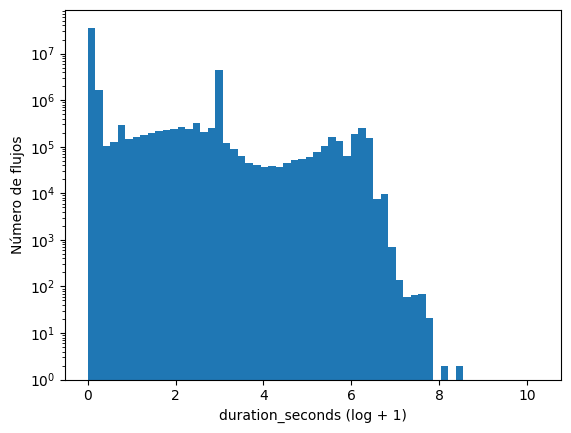
\includegraphics[width=\textwidth]{media/packet_pincer_cicddos/duration_seconds_log_x_log_y.png}
        \caption{CIC-DDoS2019}
    \end{subfigure}
    \hfill
    \begin{subfigure}[b]{0.26\textwidth}
        \centering
        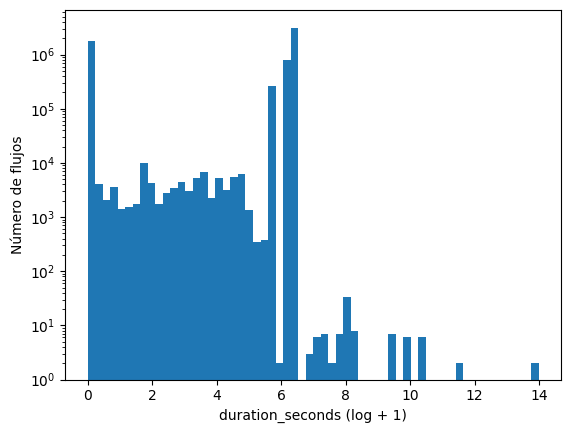
\includegraphics[width=\linewidth]{media/packet_pincer_botiot/duration_seconds_log_x_log_y.png}
        \caption{BoT-IoT}
    \end{subfigure}
    \hfill
    \begin{subfigure}[b]{0.26\textwidth}
        \centering
        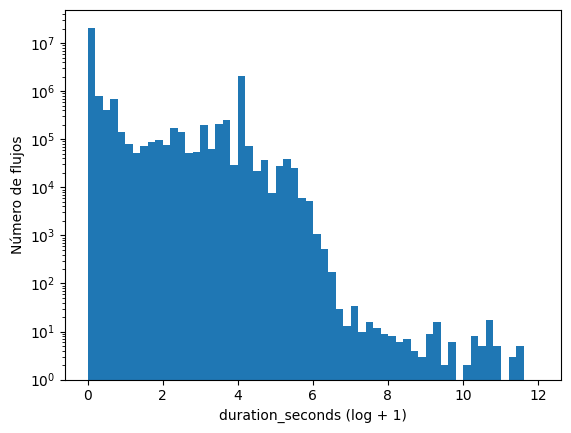
\includegraphics[width=\linewidth]{media/packet_pincer_toniot/duration_seconds_log_x_log_y.png}
        \caption{TON-IoT}
    \end{subfigure}
       \caption{Distribución de la duración de los flujos}
       \label{fig:packet_pincer_duration}
\end{figure}

\subsubsection{Recuento de paquetes}

\begin{figure}[H]
    \centering
    \hfill
    \begin{subfigure}[b]{0.26\textwidth}
        \centering
        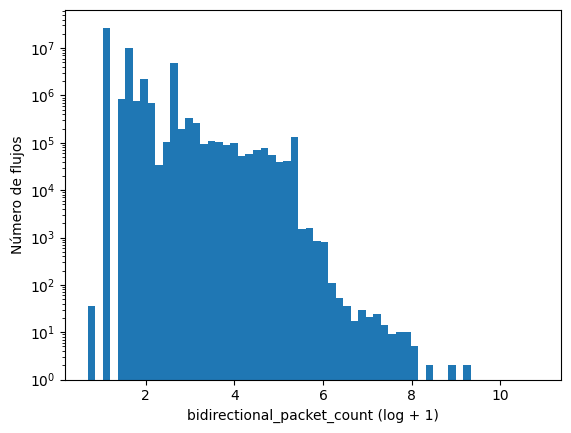
\includegraphics[width=\textwidth]{media/packet_pincer_cicddos/bidirectional_packet_count_log_x_log_y.png}
        \caption{CD (bidir.)}
        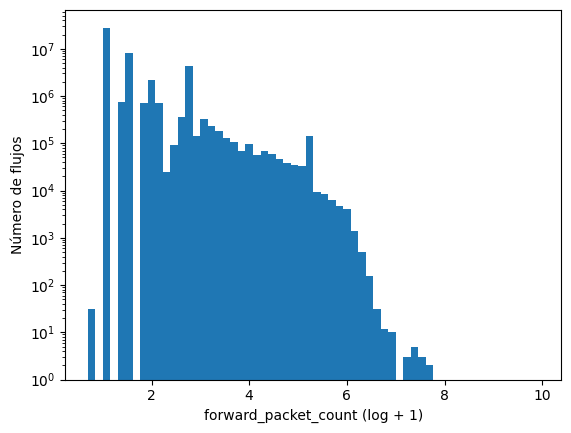
\includegraphics[width=\textwidth]{media/packet_pincer_cicddos/forward_packet_count_log_x_log_y.png}
        \caption{CD (forward)}
        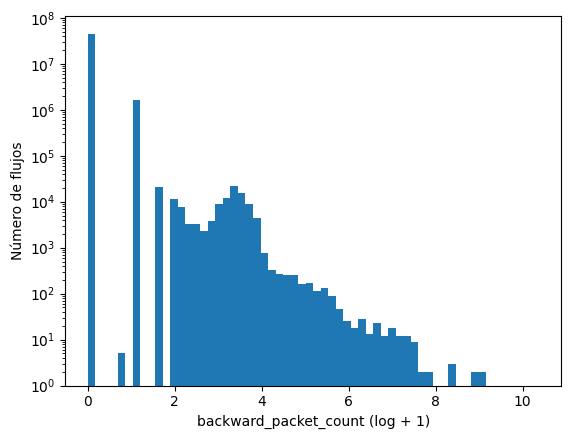
\includegraphics[width=\textwidth]{media/packet_pincer_cicddos/backward_packet_count_log_x_log_y.png}
        \caption{CD (backward)}
    \end{subfigure}
    \hfill
    \begin{subfigure}[b]{0.26\textwidth}
        \centering
        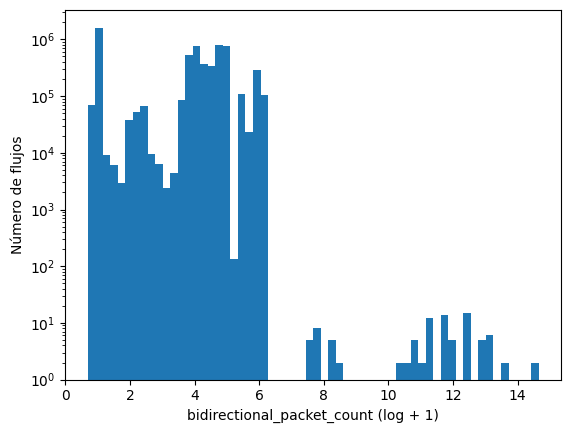
\includegraphics[width=\linewidth]{media/packet_pincer_botiot/bidirectional_packet_count_log_x_log_y.png}
        \caption{BI (bidir.)}
        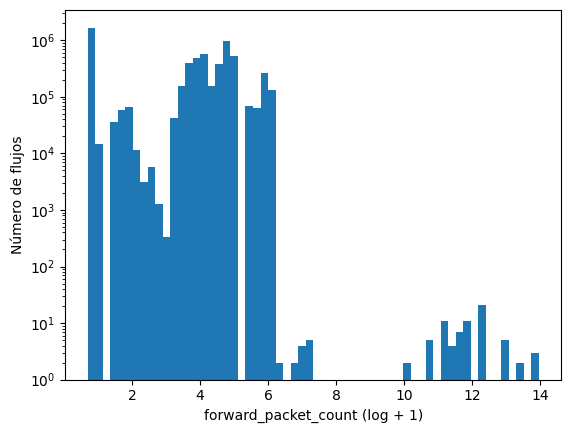
\includegraphics[width=\textwidth]{media/packet_pincer_botiot/forward_packet_count_log_x_log_y.png}
        \caption{BI (forward)}
        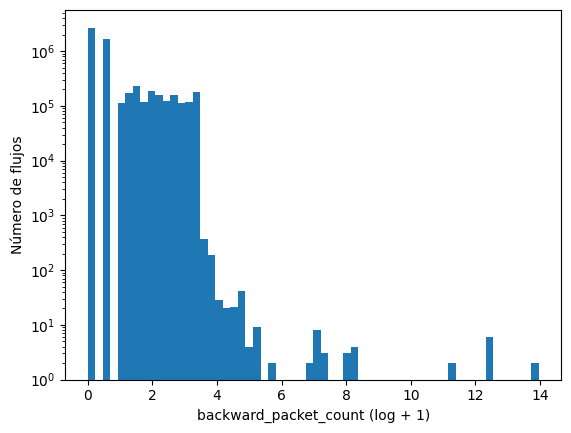
\includegraphics[width=\textwidth]{media/packet_pincer_botiot/backward_packet_count_log_x_log_y.png}
        \caption{BI (backward)}
    \end{subfigure}
    \hfill
    \begin{subfigure}[b]{0.26\textwidth}
        \centering
        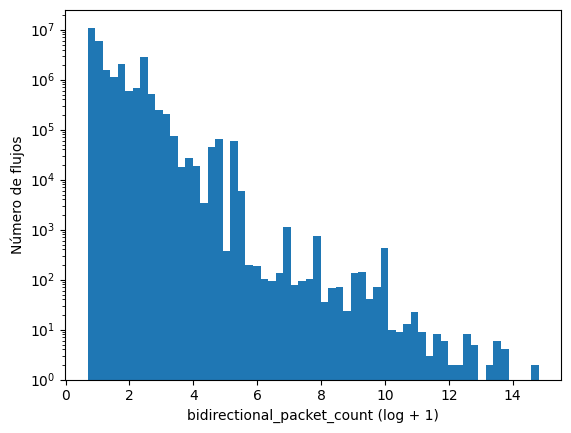
\includegraphics[width=\linewidth]{media/packet_pincer_toniot/bidirectional_packet_count_log_x_log_y.png}
        \caption{TI (bidir.)}
        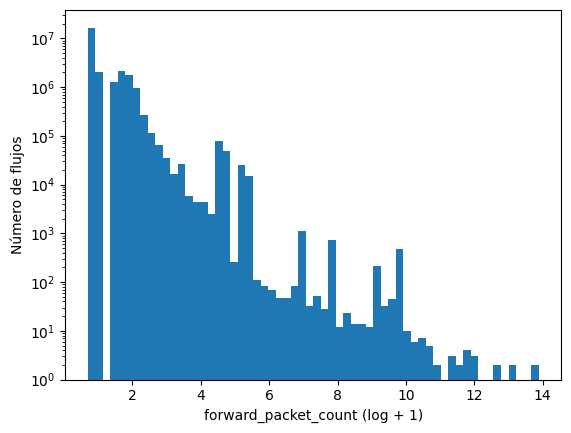
\includegraphics[width=\textwidth]{media/packet_pincer_toniot/forward_packet_count_log_x_log_y.png}
        \caption{TI (forward)}
        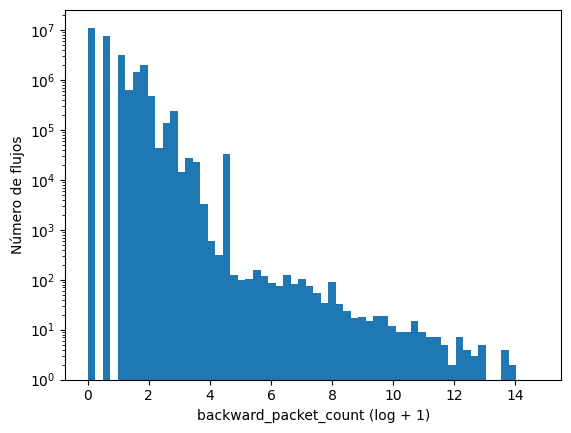
\includegraphics[width=\textwidth]{media/packet_pincer_toniot/backward_packet_count_log_x_log_y.png}
        \caption{TI (backward)}
    \end{subfigure}
    \hfill
       \caption{Distribución del número de paquetes}
       \label{fig:packet_pincer_packet_count}
\end{figure}

Podemos observar en la Figura \ref{fig:packet_pincer_packet_count} que tenemos una situación parecida al caso de la duración con el recuento de paquetes. La mayoría de los flujos tienen una cantidad de paquetes intercambiados reducida. Adicionalmente, en la mayoría hay una caída clara a partir de un punto, aunque en otros es más progresivo. Para CIC-DDoS2019 (CD en la figura) y en ToN-IoT (TI en la figura), podemos observar cierta tendencia que predice la ley de Zipf.

En este caso, para la columna del recuento de paquetes de regreso, tenemos que la cantidad de ceros es el 96.29\% (46 588 405), 44.39\% (2 697 786) y 41.71\% (11 264 084) en CIC-DDoS2019, BoT-Iot y TON-IoT, respectivamente. Las otras dos no contienen ningún cero, debido a que si fuesen cero, el flujo no aparecería en los datos procesados.

\subsubsection{Cadencia de paquetes}

\begin{figure}[H]
    \centering
    \hfill
    \begin{subfigure}[b]{0.26\textwidth}
        \centering
        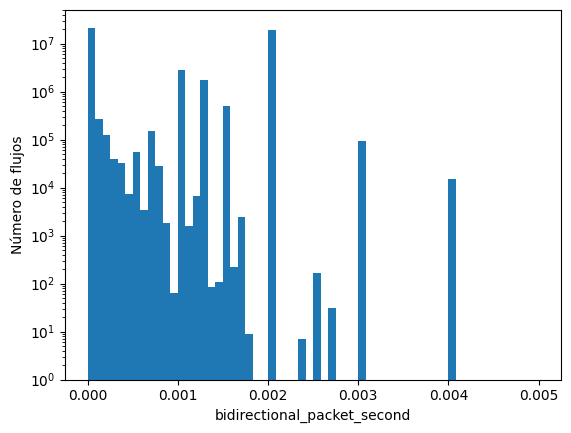
\includegraphics[width=\textwidth]{media/packet_pincer_cicddos/bidirectional_packet_second_linear_x_log_y.png}
        \caption{CD (bidir.)}
        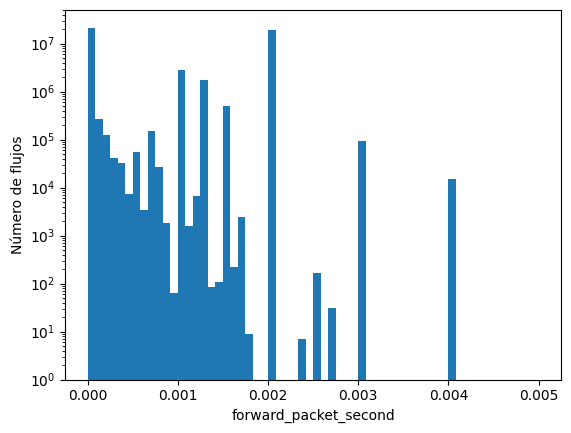
\includegraphics[width=\textwidth]{media/packet_pincer_cicddos/forward_packet_second_linear_x_log_y.png}
        \caption{CD (forward)}
        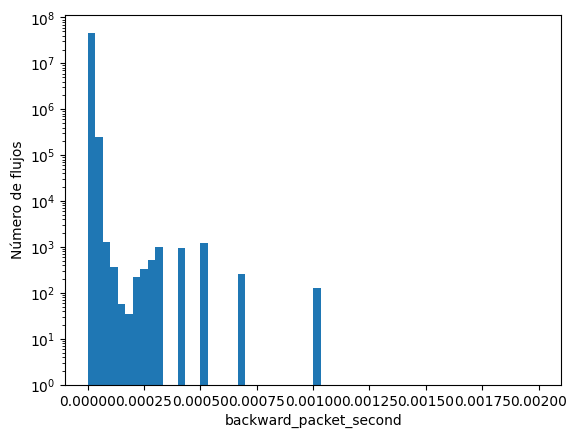
\includegraphics[width=\textwidth]{media/packet_pincer_cicddos/backward_packet_second_linear_x_log_y.png}
        \caption{CD (backward)}
    \end{subfigure}
    \hfill
    \begin{subfigure}[b]{0.26\textwidth}
        \centering
        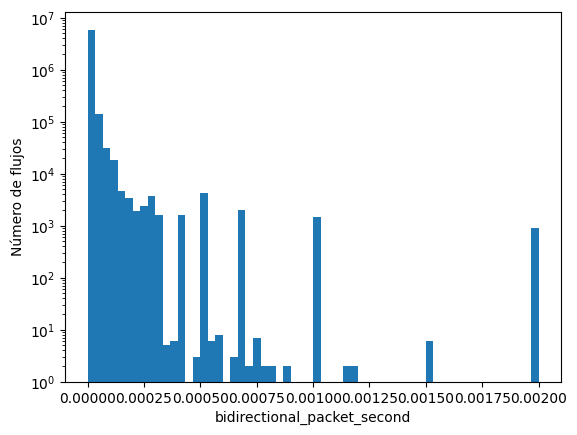
\includegraphics[width=\linewidth]{media/packet_pincer_botiot/bidirectional_packet_second_linear_x_log_y.png}
        \caption{BI (bidir.)}
        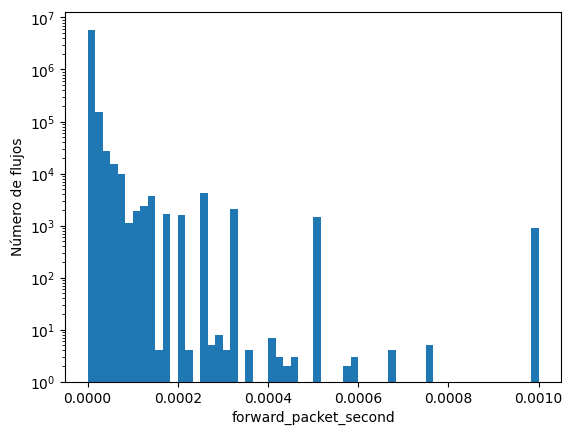
\includegraphics[width=\textwidth]{media/packet_pincer_botiot/forward_packet_second_linear_x_log_y.png}
        \caption{BI (forward)}
        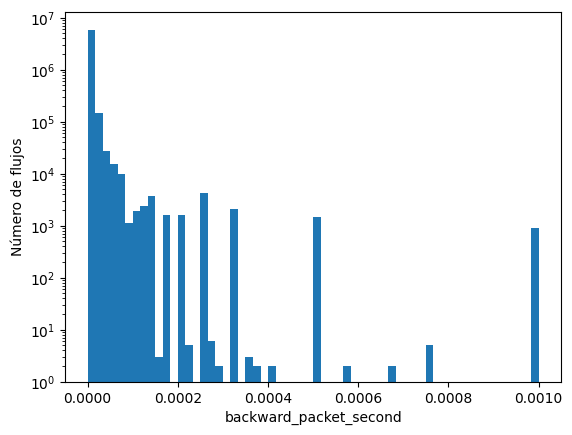
\includegraphics[width=\textwidth]{media/packet_pincer_botiot/backward_packet_second_linear_x_log_y.png}
        \caption{BI (backward)}
    \end{subfigure}
    \hfill
    \begin{subfigure}[b]{0.26\textwidth}
        \centering
        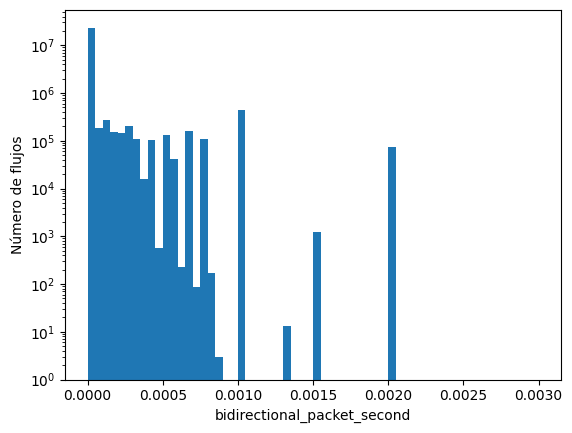
\includegraphics[width=\linewidth]{media/packet_pincer_toniot/bidirectional_packet_second_linear_x_log_y.png}
        \caption{TI (bidir.)}
        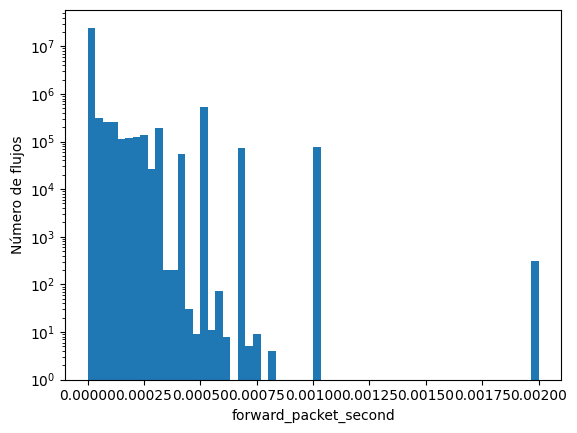
\includegraphics[width=\textwidth]{media/packet_pincer_toniot/forward_packet_second_linear_x_log_y.png}
        \caption{TI (forward)}
        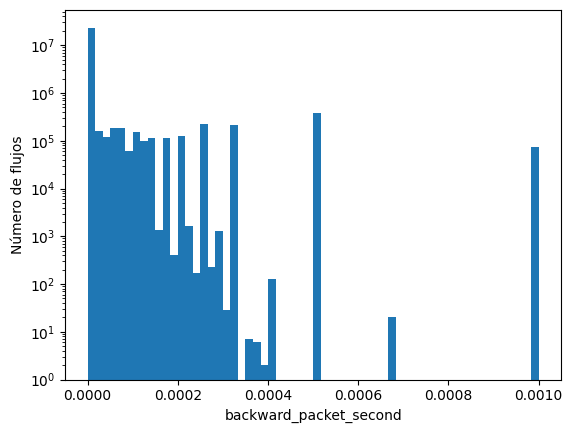
\includegraphics[width=\textwidth]{media/packet_pincer_toniot/backward_packet_second_linear_x_log_y.png}
        \caption{TI (backward)}
    \end{subfigure}
    \hfill
       \caption{Distribución de la cadencia de paquetes}
       \label{fig:packet_pincer_packet_second}
\end{figure}

La distribución de las diferentes cadencias de paquetes se puede observar en la Figura \ref{fig:packet_pincer_packet_second}. Podemos ver que la mayoría de los flujos tiene una cadencia baja, con algunos puntos con picos. En la Tabla \ref{table:packet_pincer_packet_second_zeroes} podemos ver que también hay gran cantidad de ceros en el conjunto de datos, especialmente en los \acrshort{iot} y en los casos de retorno. Es posible que esto haya sido debido a muchos paquetes que no hayan tenido respuesta.

\begin{table}[H]
    \centering
    \begin{tabular}{|c | c c c |}
        \hline
        \textbf{Conjunto de datos} & \textbf{Bidirectional} & \textbf{Forward} & \textbf{Backward} \\ \hline
        CIC-DDoS2019               & 6,97\%                 & 6,99\%           & 95,55\% \\
        Bot-IoT                    & 64,38\%                & 64,53\%          & 71,14\% \\
        TON-IoT                    & 53,10\%                & 54,44\%          & 55,27\% \\
        \hline
    \end{tabular}
    \caption{Cantidad de ceros por conjunto de datos}
    \label{table:packet_pincer_packet_second_zeroes}
\end{table}

\subsubsection{Número de bytes transmitidos por flujo}

\begin{figure}[H]
    \centering
    \hfill
    \begin{subfigure}[b]{0.26\textwidth}
        \centering
        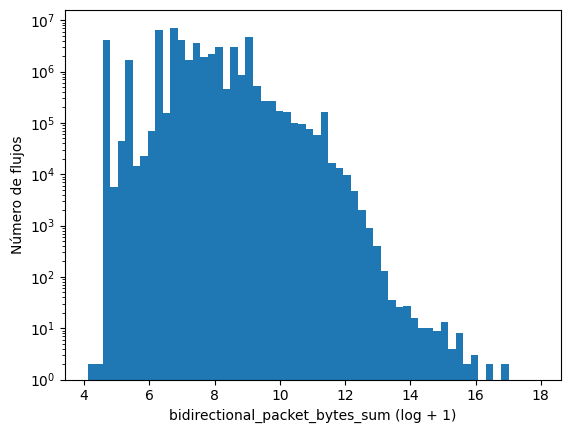
\includegraphics[width=\textwidth]{media/packet_pincer_cicddos/bidirectional_packet_bytes_sum_log_x_log_y.png}
        \caption{CD (bidir.)}
        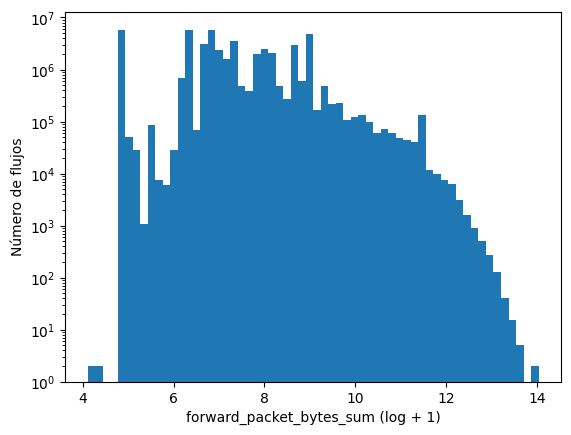
\includegraphics[width=\textwidth]{media/packet_pincer_cicddos/forward_packet_bytes_sum_log_x_log_y.png}
        \caption{CD (forward)}
        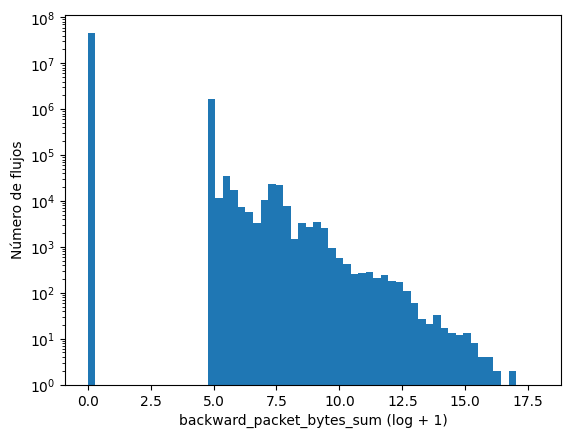
\includegraphics[width=\textwidth]{media/packet_pincer_cicddos/backward_packet_bytes_sum_log_x_log_y.png}
        \caption{CD (backward)}
    \end{subfigure}
    \hfill
    \begin{subfigure}[b]{0.26\textwidth}
        \centering
        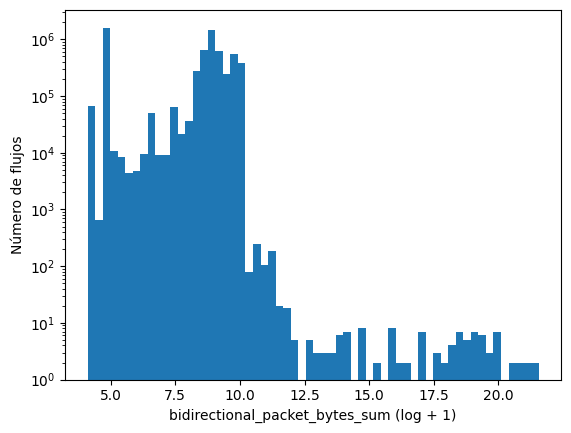
\includegraphics[width=\linewidth]{media/packet_pincer_botiot/bidirectional_packet_bytes_sum_log_x_log_y.png}
        \caption{BI (bidir.)}
        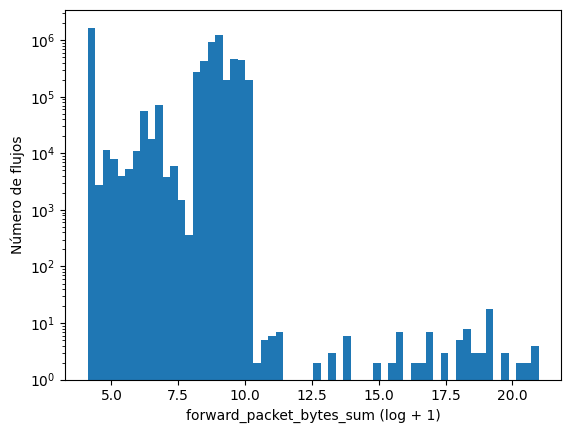
\includegraphics[width=\textwidth]{media/packet_pincer_botiot/forward_packet_bytes_sum_log_x_log_y.png}
        \caption{BI (forward)}
        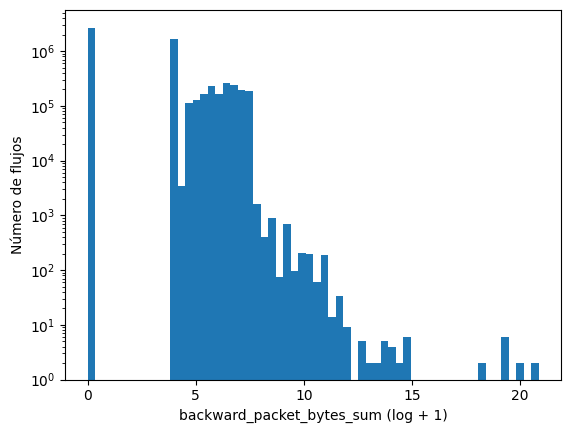
\includegraphics[width=\textwidth]{media/packet_pincer_botiot/backward_packet_bytes_sum_log_x_log_y.png}
        \caption{BI (backward)}
    \end{subfigure}
    \hfill
    \begin{subfigure}[b]{0.26\textwidth}
        \centering
        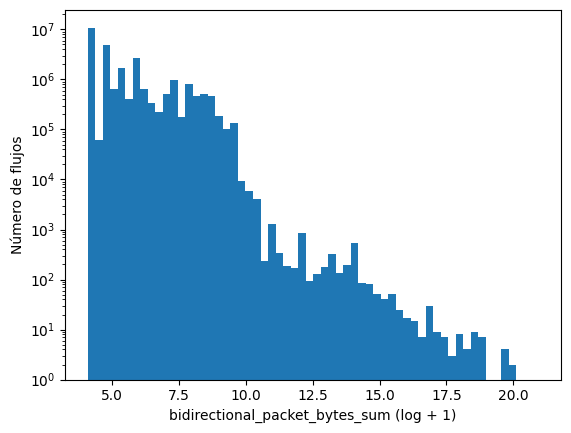
\includegraphics[width=\linewidth]{media/packet_pincer_toniot/bidirectional_packet_bytes_sum_log_x_log_y.png}
        \caption{TI (bidir.)}
        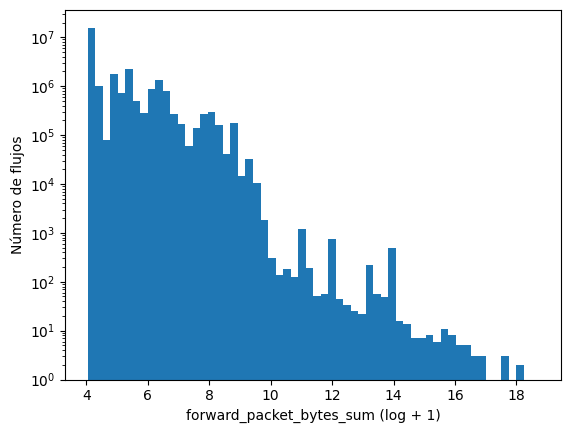
\includegraphics[width=\textwidth]{media/packet_pincer_toniot/forward_packet_bytes_sum_log_x_log_y.png}
        \caption{TI (forward)}
        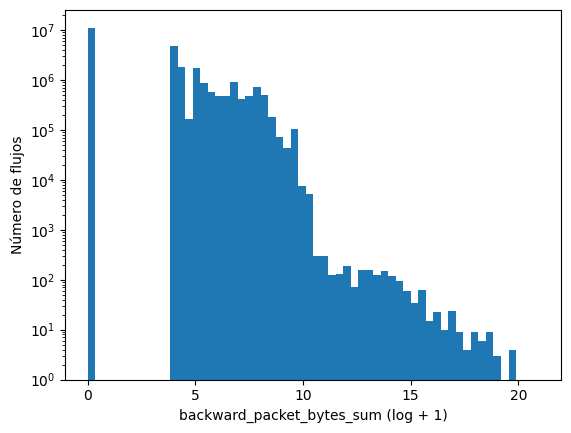
\includegraphics[width=\textwidth]{media/packet_pincer_toniot/backward_packet_bytes_sum_log_x_log_y.png}
        \caption{TI (backward)}
    \end{subfigure}
    \hfill
       \caption{Distribución de la suma de bytes transmitidas por flujo}
       \label{fig:packet_pincer_packet_bytes_sum}
\end{figure}

La distribución de las sumas totales de los bytes transmitidos por cada flujo está representada en la Figura \ref{fig:packet_pincer_packet_bytes_sum}. Podemos ver que en algunos casos la distribución parece marcada por la ley de Zipf, pero otro se asemeja más a una distribución normal al expresarlo en una gráfica log-log. Adicionalmente, en otros tenemos una caída notable a partir de cierto punto. Aparte de las peticiones que no reciben respuesta, no hay registros con ceros.

\subsubsection{Número de bytes máximos por flujo}

Si observamos las distribuciones de los bytes máximos en paquetes por flujo representadas en la Figura \ref{fig:packet_pincer_packet_bytes_max}, podemos ver que en general son similares a las del punto anterior. Sin embargo, en el caso 'backward' del conjunto de datos de CIC-DDoS2019 (subfigura \ref{fig:packet_pincer_packet_bytes_max_backward}), podemos ver cómo la 'cola' de la distribución parece haber sido cortada. Adicionalmente, los picos parecen ser menos pronunciados para los otros dos conjuntos.

\begin{figure}[H]
    \centering
    \hfill
    \begin{subfigure}[b]{0.26\textwidth}
        \centering
        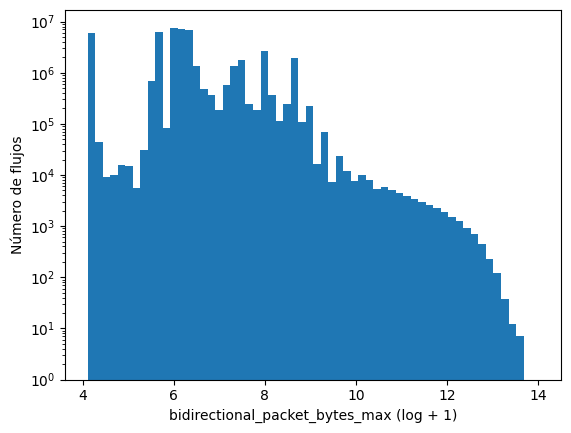
\includegraphics[width=\textwidth]{media/packet_pincer_cicddos/bidirectional_packet_bytes_max_log_x_log_y.png}
        \caption{CD (bidir.)}
        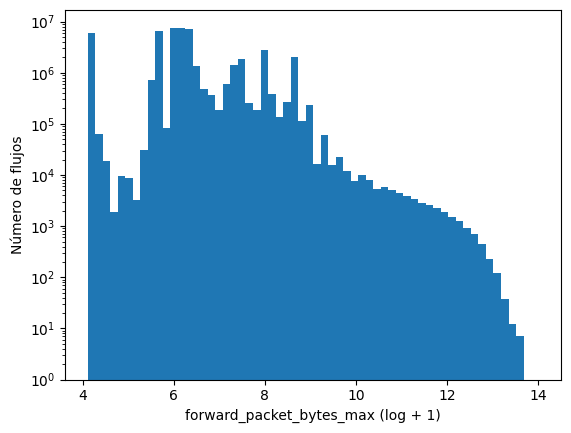
\includegraphics[width=\textwidth]{media/packet_pincer_cicddos/forward_packet_bytes_max_log_x_log_y.png}
        \caption{CD (forward)}
        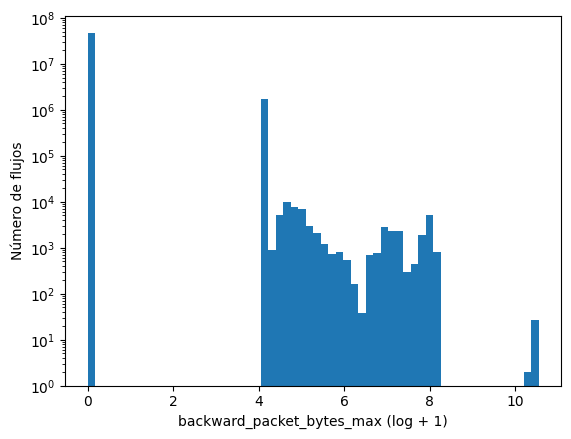
\includegraphics[width=\textwidth]{media/packet_pincer_cicddos/backward_packet_bytes_max_log_x_log_y.png}
        \caption{CD (backward)} \label{fig:packet_pincer_packet_bytes_max_backward}
    \end{subfigure}
    \hfill
    \begin{subfigure}[b]{0.26\textwidth}
        \centering
        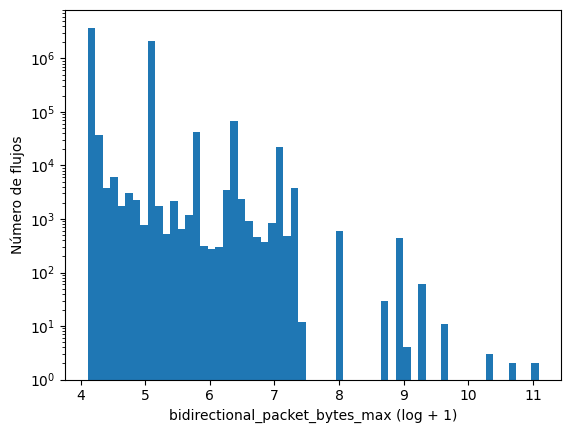
\includegraphics[width=\linewidth]{media/packet_pincer_botiot/bidirectional_packet_bytes_max_log_x_log_y.png}
        \caption{BI (bidir.)}
        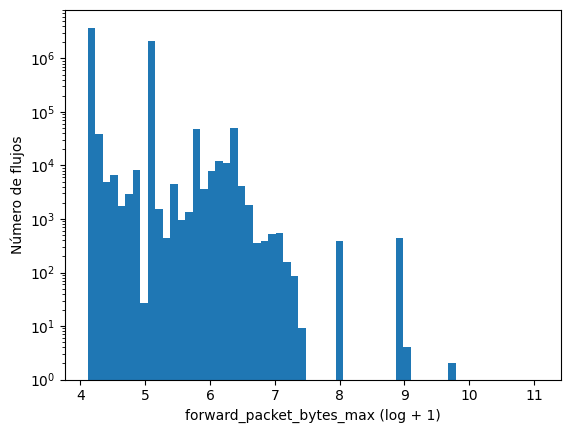
\includegraphics[width=\textwidth]{media/packet_pincer_botiot/forward_packet_bytes_max_log_x_log_y.png}
        \caption{BI (forward)}
        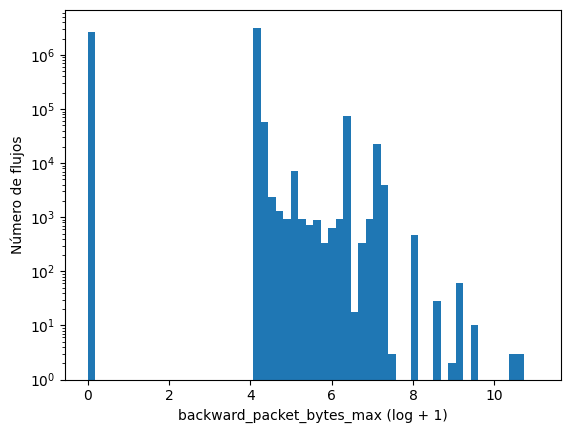
\includegraphics[width=\textwidth]{media/packet_pincer_botiot/backward_packet_bytes_max_log_x_log_y.png}
        \caption{BI (backward)}
    \end{subfigure}
    \hfill
    \begin{subfigure}[b]{0.26\textwidth}
        \centering
        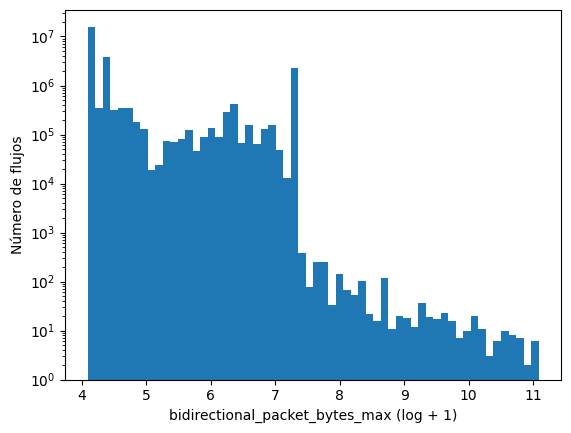
\includegraphics[width=\linewidth]{media/packet_pincer_toniot/bidirectional_packet_bytes_max_log_x_log_y.png}
        \caption{TI (bidir.)}
        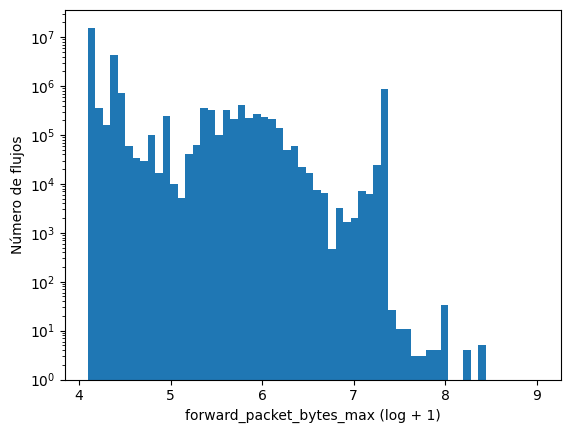
\includegraphics[width=\textwidth]{media/packet_pincer_toniot/forward_packet_bytes_max_log_x_log_y.png}
        \caption{TI (forward)}
        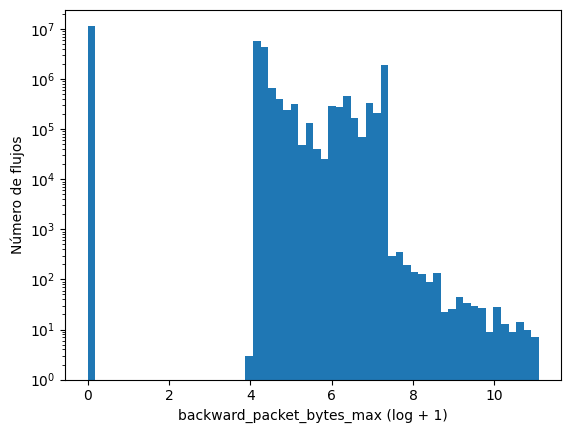
\includegraphics[width=\textwidth]{media/packet_pincer_toniot/backward_packet_bytes_max_log_x_log_y.png}
        \caption{TI (backward)}
    \end{subfigure}
    \hfill
       \caption{Distribución de los máximos bytes transmitidos en un paquete por flujo}
       \label{fig:packet_pincer_packet_bytes_max}
\end{figure}

\subsubsection{Número de bytes mínimos por flujo}

Para el caso de bytes mínimos en paquetes, podemos ver que en la Figura \ref{fig:packet_pincer_packet_bytes_min} nos encontramos con una situación al caso de los máximos. Sin embargo, para CIC-DDoS2019, el corte es en una magnitud menor (subfigura \ref{fig:packet_pincer_packet_bytes_min_backward}) y en los otros parece haber más huecos y concentraciones en ciertos puntos de la distribución.

\begin{figure}[H]
    \centering
    \hfill
    \begin{subfigure}[b]{0.26\textwidth}
        \centering
        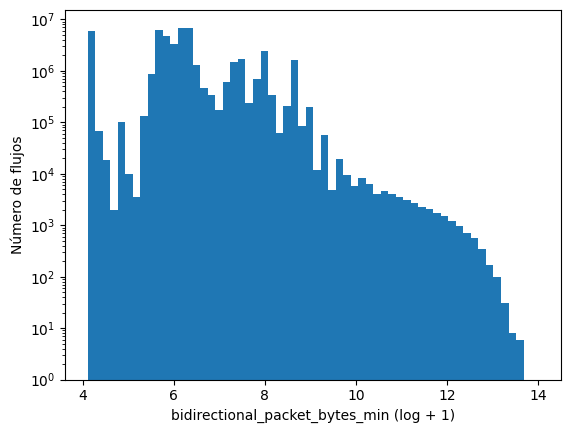
\includegraphics[width=\textwidth]{media/packet_pincer_cicddos/bidirectional_packet_bytes_min_log_x_log_y.png}
        \caption{CD (bidir.)}
        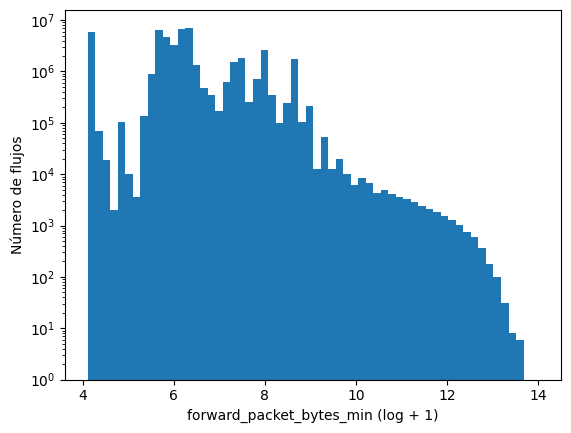
\includegraphics[width=\textwidth]{media/packet_pincer_cicddos/forward_packet_bytes_min_log_x_log_y.png}
        \caption{CD (forward)}
        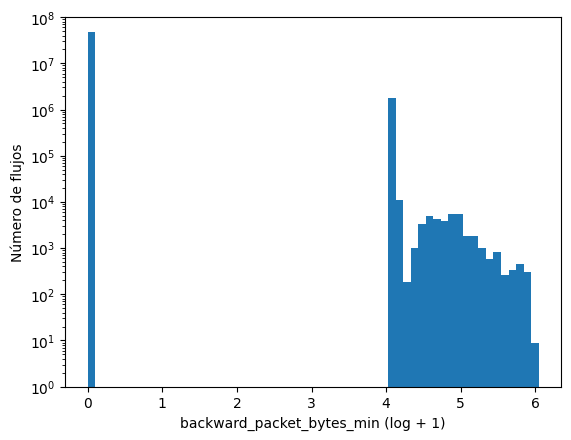
\includegraphics[width=\textwidth]{media/packet_pincer_cicddos/backward_packet_bytes_min_log_x_log_y.png}
        \caption{CD (backward)} \label{fig:packet_pincer_packet_bytes_min_backward}
    \end{subfigure}
    \hfill
    \begin{subfigure}[b]{0.26\textwidth}
        \centering
        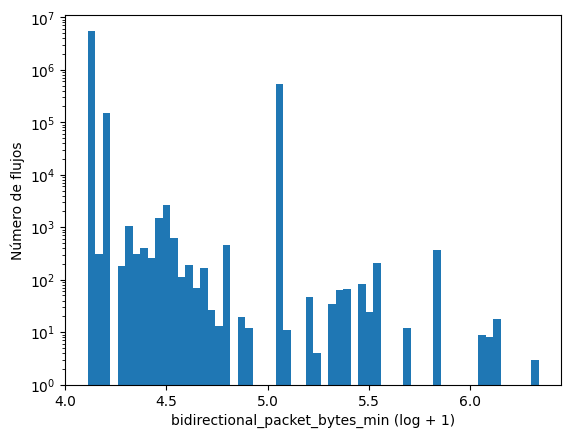
\includegraphics[width=\linewidth]{media/packet_pincer_botiot/bidirectional_packet_bytes_min_log_x_log_y.png}
        \caption{BI (bidir.)}
        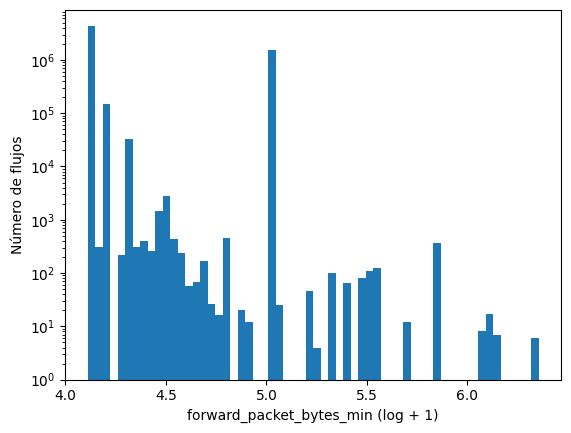
\includegraphics[width=\textwidth]{media/packet_pincer_botiot/forward_packet_bytes_min_log_x_log_y.png}
        \caption{BI (forward)}
        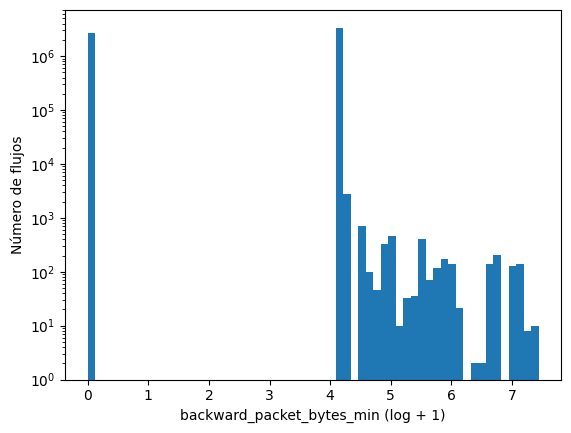
\includegraphics[width=\textwidth]{media/packet_pincer_botiot/backward_packet_bytes_min_log_x_log_y.png}
        \caption{BI (backward)}
    \end{subfigure}
    \hfill
    \begin{subfigure}[b]{0.26\textwidth}
        \centering
        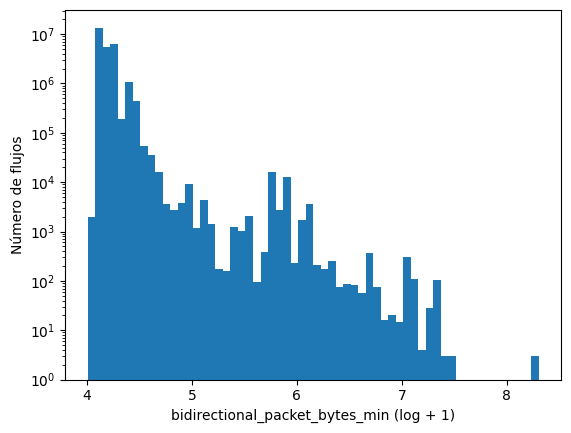
\includegraphics[width=\linewidth]{media/packet_pincer_toniot/bidirectional_packet_bytes_min_log_x_log_y.png}
        \caption{TI (bidir.)}
        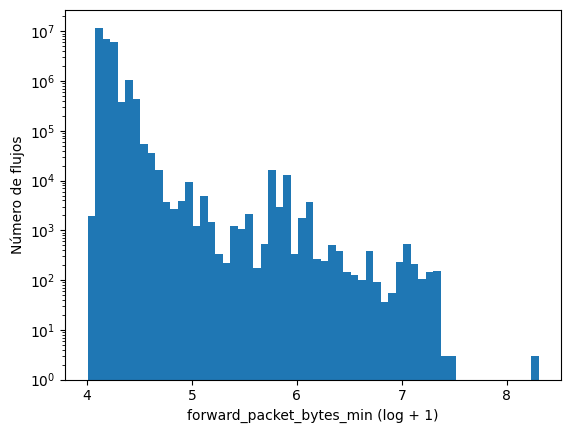
\includegraphics[width=\textwidth]{media/packet_pincer_toniot/forward_packet_bytes_min_log_x_log_y.png}
        \caption{TI (forward)}
        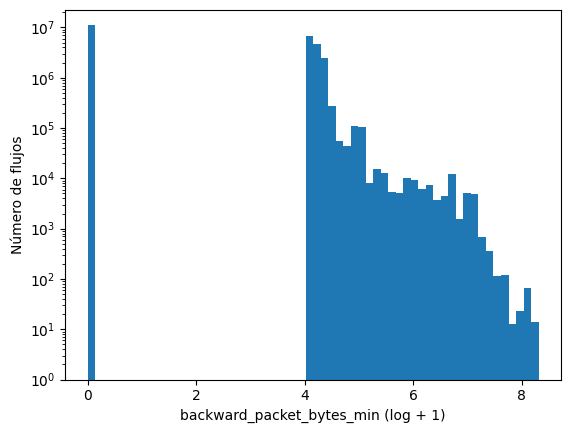
\includegraphics[width=\textwidth]{media/packet_pincer_toniot/backward_packet_bytes_min_log_x_log_y.png}
        \caption{TI (backward)}
    \end{subfigure}
    \hfill
       \caption{Distribución de los mínimos bytes transmitidos en un paquete por flujo}
       \label{fig:packet_pincer_packet_bytes_min}
\end{figure}

\subsubsection{Número de bytes medio por flujo}

Las distribuciones de los bytes medios de la Figura \ref{fig:packet_pincer_packet_bytes_mean} se asemejan a las de los recuentos de los bytes totales, pero suavizadas. Podemos ver que, en el caso bidireccional de TON-IoT (subfigura \ref{fig:packet_pincer_packet_bytes_mean_ti_bidir}), la gráfica se mantiene en número de flujos alto durante un mayor rango de medias antes de caer.

\begin{figure}[H]
    \centering
    \hfill
    \begin{subfigure}[b]{0.26\textwidth}
        \centering
        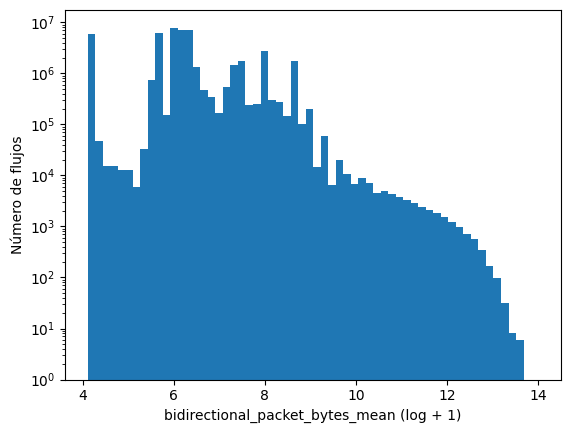
\includegraphics[width=\textwidth]{media/packet_pincer_cicddos/bidirectional_packet_bytes_mean_log_x_log_y.png}
        \caption{CD (bidir.)}
        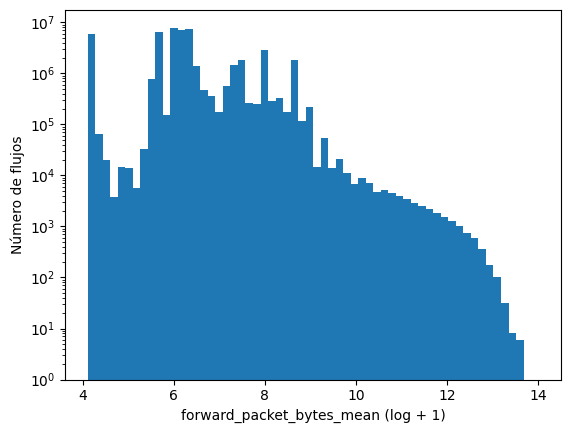
\includegraphics[width=\textwidth]{media/packet_pincer_cicddos/forward_packet_bytes_mean_log_x_log_y.png}
        \caption{CD (forward)}
        \includegraphics[width=\textwidth]{media/packet_pincer_cicddos/backward_packet_bytes_mean_log_x_log_y.png}
        \caption{CD (backward)}
    \end{subfigure}
    \hfill
    \begin{subfigure}[b]{0.26\textwidth}
        \centering
        \includegraphics[width=\linewidth]{media/packet_pincer_botiot/bidirectional_packet_bytes_mean_log_x_log_y.png}
        \caption{BI (bidir.)}
        \includegraphics[width=\textwidth]{media/packet_pincer_botiot/forward_packet_bytes_mean_log_x_log_y.png}
        \caption{BI (forward)}
        \includegraphics[width=\textwidth]{media/packet_pincer_botiot/backward_packet_bytes_mean_log_x_log_y.png}
        \caption{BI (backward)}
    \end{subfigure}
    \hfill
    \begin{subfigure}[b]{0.26\textwidth}
        \centering
        \includegraphics[width=\linewidth]{media/packet_pincer_toniot/bidirectional_packet_bytes_mean_log_x_log_y.png}
        \caption{TI (bidir.)} \label{fig:packet_pincer_packet_bytes_mean_ti_bidir}
        \includegraphics[width=\textwidth]{media/packet_pincer_toniot/forward_packet_bytes_mean_log_x_log_y.png}
        \caption{TI (forward)}
        \includegraphics[width=\textwidth]{media/packet_pincer_toniot/backward_packet_bytes_mean_log_x_log_y.png}
        \caption{TI (backward)}
    \end{subfigure}
    \hfill
       \caption{Distribución de los bytes medios transmitidos en un paquete por flujo}
       \label{fig:packet_pincer_packet_bytes_mean}
\end{figure}

\subsubsection{Desviación estándar del número de bytes por flujo}

Las distribuciones de las diferentes desviaciones estándar son variadas. Tenemos en muchos casos donde la desviación es 0, la cual puede ser causada por flujos con paquetes muy iguales o los casos donde no se transmite nada, ya que se asigna 0 en ese caso. De todas formas, para todos los casos, donde no son 0, hay una variedad de distribuciones. En el caso de CIC-DDoS2019, se mantiene el estilo de sus distribuciones anteriores en el caso bidireccional y hacia el receptor inicial. Para el caso hacia el transmisor inicial (subfigura \ref{fig:packet_pincer_packet_bytes_std_cd_bw}) está invertida, teniendo mucha variabilidad en la cantidad total de bytes enviados. La gran diferencia de variabilidad es quizá debido a los efectos del control de congestión de las transmisiones. Dependiendo del estado de la red, los diferentes dispositivos transmitirán de una forma más constante y predecible y en otras se tendrán que ir adaptando a tiempo real al nivel de congestión.

\begin{figure}[H]
    \centering
    \hfill
    \begin{subfigure}[b]{0.26\textwidth}
        \centering
        \includegraphics[width=\textwidth]{media/packet_pincer_cicddos/bidirectional_packet_bytes_std_log_x_log_y.png}
        \caption{CD (bidir.)}
        \includegraphics[width=\textwidth]{media/packet_pincer_cicddos/forward_packet_bytes_std_log_x_log_y.png}
        \caption{CD (forward)}
        \includegraphics[width=\textwidth]{media/packet_pincer_cicddos/backward_packet_bytes_std_log_x_log_y.png}
        \caption{CD (backward)} \label{fig:packet_pincer_packet_bytes_std_cd_bw}
    \end{subfigure}
    \hfill
    \begin{subfigure}[b]{0.26\textwidth}
        \centering
        \includegraphics[width=\linewidth]{media/packet_pincer_botiot/bidirectional_packet_bytes_std_log_x_log_y.png}
        \caption{BI (bidir.)}
        \includegraphics[width=\textwidth]{media/packet_pincer_botiot/forward_packet_bytes_std_log_x_log_y.png}
        \caption{BI (forward)}
        \includegraphics[width=\textwidth]{media/packet_pincer_botiot/backward_packet_bytes_std_log_x_log_y.png}
        \caption{BI (backward)}
    \end{subfigure}
    \hfill
    \begin{subfigure}[b]{0.26\textwidth}
        \centering
        \includegraphics[width=\linewidth]{media/packet_pincer_toniot/bidirectional_packet_bytes_std_log_x_log_y.png}
        \caption{TI (bidir.)}
        \includegraphics[width=\textwidth]{media/packet_pincer_toniot/forward_packet_bytes_std_log_x_log_y.png}
        \caption{TI (forward)}
        \includegraphics[width=\textwidth]{media/packet_pincer_toniot/backward_packet_bytes_std_log_x_log_y.png}
        \caption{TI (backward)}
    \end{subfigure}
    \hfill
       \caption{Desviación estándard del número de bytes transmitidos en un paquete por flujo}
       \label{fig:packet_pincer_packet_bytes_std}
\end{figure}

\subsubsection{Balance entre subida y bajada}

El balance o la razón entre la subida y bajada consiste en dividir la cantidad de bytes enviados por el receptor inicial entre los enviados por el iniciador de la comunicación. De esta manera, se puede inferir si la comunicación es principalmente de bajada (un valor inferior a 1), de subida (un valor superior a 1) o hay una comunicación a iguales. En el primer caso, se puede dar al visitar la web o descargar archivos. El segundo en casos donde se suban datos, como subir fotos a un servicio Cloud. Finalmente, el tercero podría consistir en, por ejemplo, en una llamada de voz o videoconferencia. 

Podemos ver en la Figura \ref{fig:packet_pincer_down_up_bytes_ratio} que la gran mayoría de comunicaciones se concentran en la parte baja del gráfico, indicando que suelen ser o de bajada o la cantidad de datos enviados no suele ser muy grande. Sin embargo, hay una cantidad relevante de flujos en la que el emisor de la comunicación envía muchos más datos de los que recibe. Esto puede estar relacionado con posibles ataques, donde las comunicaciones normales tienen un ratio más bajo.

\begin{figure}[H]
    \centering
    \begin{subfigure}[b]{0.32\textwidth}
        \centering
        \includegraphics[width=\textwidth]{media/packet_pincer_cicddos/down_up_bytes_ratio_log_x_log_y.png}
        \caption{CIC-DDoS2019}
    \end{subfigure}
    \hfill
    \begin{subfigure}[b]{0.32\textwidth}
        \centering
        \includegraphics[width=\linewidth]{media/packet_pincer_botiot/down_up_bytes_ratio_log_x_log_y.png}
        \caption{BoT-IoT}
    \end{subfigure}
    \hfill
    \begin{subfigure}[b]{0.32\textwidth}
        \centering
        \includegraphics[width=\linewidth]{media/packet_pincer_toniot/down_up_bytes_ratio_log_x_log_y.png}
        \caption{TON-IoT}
    \end{subfigure}
       \caption{Distribución del balance de los flujos}
       \label{fig:packet_pincer_down_up_bytes_ratio}
\end{figure}

\subsubsection{Cadencia de datos}

\begin{figure}[H]
    \centering
    \hfill
    \begin{subfigure}[b]{0.26\textwidth}
        \centering
        \includegraphics[width=\textwidth]{media/packet_pincer_cicddos/bidirectional_bytes_s_log_x_log_y.png}
        \caption{CD (bidir.)}
        \includegraphics[width=\textwidth]{media/packet_pincer_cicddos/forward_bytes_s_log_x_log_y.png}
        \caption{CD (forward)}
        \includegraphics[width=\textwidth]{media/packet_pincer_cicddos/backward_bytes_s_log_x_log_y.png}
        \caption{CD (backward)}
    \end{subfigure}
    \hfill
    \begin{subfigure}[b]{0.26\textwidth}
        \centering
        \includegraphics[width=\linewidth]{media/packet_pincer_botiot/bidirectional_bytes_s_log_x_log_y.png}
        \caption{BI (bidir.)}
        \includegraphics[width=\textwidth]{media/packet_pincer_botiot/forward_bytes_s_log_x_log_y.png}
        \caption{BI (forward)}
        \includegraphics[width=\textwidth]{media/packet_pincer_botiot/backward_bytes_s_log_x_log_y.png}
        \caption{BI (backward)}
    \end{subfigure}
    \hfill
    \begin{subfigure}[b]{0.26\textwidth}
        \centering
        \includegraphics[width=\linewidth]{media/packet_pincer_toniot/bidirectional_bytes_s_log_x_log_y.png}
        \caption{TI (bidir.)}
        \includegraphics[width=\textwidth]{media/packet_pincer_toniot/forward_bytes_s_log_x_log_y.png}
        \caption{TI (forward)}
        \includegraphics[width=\textwidth]{media/packet_pincer_toniot/backward_bytes_s_log_x_log_y.png}
        \caption{TI (backward)}
    \end{subfigure}
    \hfill
       \caption{Cadencia de bytes medios por flujo}
       \label{fig:packet_pincer_bytes_s}
\end{figure}

En la Figura \ref{fig:packet_pincer_bytes_s} podemos ver la distribución de las diferentes cadencias medias de bytes transmitidos por flujos. Podemos observar que hay mayor variedad en el caso de CIC-DDoS2019, mientras que en las otras los valores son más bajos y se encuentran más concentrados. Estos valores pueden aportar información sobre transmisiones en las que haya habido mayor o menor actividad.

\subsubsection{Tiempo de llegada máxima}

\begin{figure}[H]
    \centering
    \hfill
    \begin{subfigure}[b]{0.26\textwidth}
        \centering
        \includegraphics[width=\textwidth]{media/packet_pincer_cicddos/bidirectional_inter_arrival_time_max_log_x_log_y.png}
        \caption{CD (bidir.)}
        \includegraphics[width=\textwidth]{media/packet_pincer_cicddos/forward_inter_arrival_time_max_log_x_log_y.png}
        \caption{CD (forward)}
        \includegraphics[width=\textwidth]{media/packet_pincer_cicddos/backward_inter_arrival_time_max_log_x_log_y.png}
        \caption{CD (backward)}
    \end{subfigure}
    \hfill
    \begin{subfigure}[b]{0.26\textwidth}
        \centering
        \includegraphics[width=\linewidth]{media/packet_pincer_botiot/bidirectional_inter_arrival_time_max_log_x_log_y.png}
        \caption{BI (bidir.)}
        \includegraphics[width=\textwidth]{media/packet_pincer_botiot/forward_inter_arrival_time_max_log_x_log_y.png}
        \caption{BI (forward)}
        \includegraphics[width=\textwidth]{media/packet_pincer_botiot/backward_inter_arrival_time_max_log_x_log_y.png}
        \caption{BI (backward)}
    \end{subfigure}
    \hfill
    \begin{subfigure}[b]{0.26\textwidth}
        \centering
        \includegraphics[width=\linewidth]{media/packet_pincer_toniot/bidirectional_inter_arrival_time_max_log_x_log_y.png}
        \caption{TI (bidir.)}
        \includegraphics[width=\textwidth]{media/packet_pincer_toniot/forward_inter_arrival_time_max_log_x_log_y.png}
        \caption{TI (forward)}
        \includegraphics[width=\textwidth]{media/packet_pincer_toniot/backward_inter_arrival_time_max_log_x_log_y.png}
        \caption{TI (backward)}
    \end{subfigure}
    \hfill
       \caption{Distribución del tiempo de llegada máxima entre paquetes}
       \label{fig:packet_pincer_inter_arrival_time_max}
\end{figure}

La distribución de los tiempos de llegada máxima entre paquetes la podemos observar en la Figura \ref{fig:packet_pincer_inter_arrival_time_max}. Podemos ver que en los casos de CIC-DDoS2019 y TON-IOT, aparte de los ceros, la distribución de tiempos se encuentra relativamente repartida. En cambio, en BoT-IoT hay una acumulación clara en cierto punto de la gráfica.

\subsubsection{Tiempo de llegada mínima}

\begin{figure}[H]
    \centering
    \hfill
    \begin{subfigure}[b]{0.26\textwidth}
        \centering
        \includegraphics[width=\textwidth]{media/packet_pincer_cicddos/bidirectional_inter_arrival_time_min_log_x_log_y.png}
        \caption{CD (bidir.)}
        \includegraphics[width=\textwidth]{media/packet_pincer_cicddos/forward_inter_arrival_time_min_log_x_log_y.png}
        \caption{CD (forward)}
        \includegraphics[width=\textwidth]{media/packet_pincer_cicddos/backward_inter_arrival_time_min_log_x_log_y.png}
        \caption{CD (backward)}
    \end{subfigure}
    \hfill
    \begin{subfigure}[b]{0.26\textwidth}
        \centering
        \includegraphics[width=\linewidth]{media/packet_pincer_botiot/bidirectional_inter_arrival_time_min_log_x_log_y.png}
        \caption{BI (bidir.)}
        \includegraphics[width=\textwidth]{media/packet_pincer_botiot/forward_inter_arrival_time_min_log_x_log_y.png}
        \caption{BI (forward)}
        \includegraphics[width=\textwidth]{media/packet_pincer_botiot/backward_inter_arrival_time_min_log_x_log_y.png}
        \caption{BI (backward)} \label{fig:packet_pincer_inter_arrival_time_min_bi_min}
    \end{subfigure}
    \hfill
    \begin{subfigure}[b]{0.26\textwidth}
        \centering
        \includegraphics[width=\linewidth]{media/packet_pincer_toniot/bidirectional_inter_arrival_time_min_log_x_log_y.png}
        \caption{TI (bidir.)}
        \includegraphics[width=\textwidth]{media/packet_pincer_toniot/forward_inter_arrival_time_min_log_x_log_y.png}
        \caption{TI (forward)}
        \includegraphics[width=\textwidth]{media/packet_pincer_toniot/backward_inter_arrival_time_min_log_x_log_y.png}
        \caption{TI (backward)}
    \end{subfigure}
    \hfill
       \caption{Distribución del tiempo de llegada mínima entre paquetes}
       \label{fig:packet_pincer_inter_arrival_time_min}
\end{figure}

Para el caso de las llegadas mínimas entre paquetes, como podemos ver en la Figura \ref{fig:packet_pincer_inter_arrival_time_min}, tenemos que las distribuciones en BoT-Iot y TON-IoT son similares. Sin embargo, sin contar los ceros, en CIC-DDoS2019 tenemos que el caso bidireccional y hacia el receptor inicial tenemos mayor cantidad en la parte alta. Adicionalmente, con BoT-IoT no tenemos el mismo pico en para el caso 'backwards' (subfigura \ref{fig:packet_pincer_inter_arrival_time_min_bi_min})

\subsubsection{Tiempo de llegada media}

Si observamos las distribuciones del tiempo de llegada media de la Figura \ref{fig:packet_pincer_inter_arrival_time_mean}, sin tener en cuenta los ceros, podemos observar que en general hay bastante variedad entre los diferentes flujos. De todas maneras, en el caso de BoT-IoT hay mayor agrupación en la parte baja en el caso bidireccional y hacia el receptor inicial.

\begin{figure}[H]
    \centering
    \hfill
    \begin{subfigure}[b]{0.32\textwidth}
        \centering
        \includegraphics[width=\textwidth]{media/packet_pincer_cicddos/bidirectional_inter_arrival_time_mean_log_x_log_y.png}
        \caption{CD (bidir.)}
        \includegraphics[width=\textwidth]{media/packet_pincer_cicddos/forward_inter_arrival_time_mean_log_x_log_y.png}
        \caption{CD (forward)}
        \includegraphics[width=\textwidth]{media/packet_pincer_cicddos/backward_inter_arrival_time_mean_log_x_log_y.png}
        \caption{CD (backward)}
    \end{subfigure}
    \hfill
    \begin{subfigure}[b]{0.32\textwidth}
        \centering
        \includegraphics[width=\linewidth]{media/packet_pincer_botiot/bidirectional_inter_arrival_time_mean_log_x_log_y.png}
        \caption{BI (bidir.)}
        \includegraphics[width=\textwidth]{media/packet_pincer_botiot/forward_inter_arrival_time_mean_log_x_log_y.png}
        \caption{BI (forward)}
        \includegraphics[width=\textwidth]{media/packet_pincer_botiot/backward_inter_arrival_time_mean_log_x_log_y.png}
        \caption{BI (backward)}
    \end{subfigure}
    \hfill
    \begin{subfigure}[b]{0.32\textwidth}
        \centering
        \includegraphics[width=\linewidth]{media/packet_pincer_toniot/bidirectional_inter_arrival_time_mean_log_x_log_y.png}
        \caption{TI (bidir.)}
        \includegraphics[width=\textwidth]{media/packet_pincer_toniot/forward_inter_arrival_time_mean_log_x_log_y.png}
        \caption{TI (forward)}
        \includegraphics[width=\textwidth]{media/packet_pincer_toniot/backward_inter_arrival_time_mean_log_x_log_y.png}
        \caption{TI (backward)}
    \end{subfigure}
    \hfill
       \caption{Distribución de la media del tiempo de llegada entre paquetes}
       \label{fig:packet_pincer_inter_arrival_time_mean}
\end{figure}

\subsubsection{Desviación estándar de los tiempos de llegada}

Para el caso de la desviación estándar, tenemos un caso parecido a las medias como podemos ver en la Figura \ref{fig:packet_pincer_inter_arrival_time_std}. De todas maneras, las magnitudes son algo menores y la distribución está más desplazadas hacia la izquierda. 

Este valor puede aportar información como en otros casos de la situación de la congestión de la red y caracterizar mejor el flujo en cuestión. Si los tiempos de llegada varían mucho, puede ser señal de una conexión inestable o, en caso de ser un ataque, sobre el intentar aparentar tener una conexión inestable para consumir recursos del sistema receptor.

\begin{figure}[H]
    \centering
    \hfill
    \begin{subfigure}[b]{0.26\textwidth}
        \centering
        \includegraphics[width=\textwidth]{media/packet_pincer_cicddos/bidirectional_inter_arrival_time_std_log_x_log_y.png}
        \caption{CD (bidir.)}
        \includegraphics[width=\textwidth]{media/packet_pincer_cicddos/forward_inter_arrival_time_std_log_x_log_y.png}
        \caption{CD (forward)}
        \includegraphics[width=\textwidth]{media/packet_pincer_cicddos/backward_inter_arrival_time_std_log_x_log_y.png}
        \caption{CD (backward)}
    \end{subfigure}
    \hfill
    \begin{subfigure}[b]{0.26\textwidth}
        \centering
        \includegraphics[width=\linewidth]{media/packet_pincer_botiot/bidirectional_inter_arrival_time_std_log_x_log_y.png}
        \caption{BI (bidir.)}
        \includegraphics[width=\textwidth]{media/packet_pincer_botiot/forward_inter_arrival_time_std_log_x_log_y.png}
        \caption{BI (forward)}
        \includegraphics[width=\textwidth]{media/packet_pincer_botiot/backward_inter_arrival_time_std_log_x_log_y.png}
        \caption{BI (backward)}
    \end{subfigure}
    \hfill
    \begin{subfigure}[b]{0.26\textwidth}
        \centering
        \includegraphics[width=\linewidth]{media/packet_pincer_toniot/bidirectional_inter_arrival_time_std_log_x_log_y.png}
        \caption{TI (bidir.)}
        \includegraphics[width=\textwidth]{media/packet_pincer_toniot/forward_inter_arrival_time_std_log_x_log_y.png}
        \caption{TI (forward)}
        \includegraphics[width=\textwidth]{media/packet_pincer_toniot/backward_inter_arrival_time_std_log_x_log_y.png}
        \caption{TI (backward)}
    \end{subfigure}
    \hfill
       \caption{Distribución de las distribuciones estándar del tiempo de llegada}
       \label{fig:packet_pincer_inter_arrival_time_std}
\end{figure}

\subsubsection{Flags CWR, ECE y URG en cabecera TCP}

Podemos ver en Figura \ref{fig:packet_pincer_bidirectional_tcp_cwr_flags_count}, Figura \ref{fig:packet_pincer_bidirectional_tcp_ece_flags_count} y Figura \ref{fig:packet_pincer_bidirectional_tcp_urg_flags_count} que apenas tenemos flujos que tengan las flags CWR, ECE o URG activas.

\begin{figure}[H]
    \centering
    \begin{subfigure}[b]{0.32\textwidth}
        \centering
        \includegraphics[width=\textwidth]{media/packet_pincer_cicddos/bidirectional_tcp_cwr_flags_count_linear_x_log_y.png}
        \caption{CIC-DDoS2019}
    \end{subfigure}
    \hfill
    \begin{subfigure}[b]{0.32\textwidth}
        \centering
        \includegraphics[width=\linewidth]{media/packet_pincer_botiot/bidirectional_tcp_cwr_flags_count_linear_x_log_y.png}
        \caption{BoT-IoT}
    \end{subfigure}
    \hfill
    \begin{subfigure}[b]{0.32\textwidth}
        \centering
        \includegraphics[width=\linewidth]{media/packet_pincer_toniot/bidirectional_tcp_cwr_flags_count_linear_x_log_y.png}
        \caption{TON-IoT}
    \end{subfigure}
       \caption{Distribución de recuentos de paquetes con la flag CWR en \acrshort{tcp} activa}
       \label{fig:packet_pincer_bidirectional_tcp_cwr_flags_count}
\end{figure}

\begin{figure}[H]
    \centering
    \begin{subfigure}[b]{0.32\textwidth}
        \centering
        \includegraphics[width=\textwidth]{media/packet_pincer_cicddos/bidirectional_tcp_ece_flags_count_linear_x_log_y.png}
        \caption{CIC-DDoS2019}
    \end{subfigure}
    \hfill
    \begin{subfigure}[b]{0.32\textwidth}
        \centering
        \includegraphics[width=\linewidth]{media/packet_pincer_botiot/bidirectional_tcp_ece_flags_count_linear_x_log_y.png}
        \caption{BoT-IoT}
    \end{subfigure}
    \hfill
    \begin{subfigure}[b]{0.32\textwidth}
        \centering
        \includegraphics[width=\linewidth]{media/packet_pincer_toniot/bidirectional_tcp_ece_flags_count_linear_x_log_y.png}
        \caption{TON-IoT}
    \end{subfigure}
       \caption{Distribución de recuentos de paquetes con la flag ECE en \acrshort{tcp} activa}
       \label{fig:packet_pincer_bidirectional_tcp_ece_flags_count}
\end{figure}

\begin{figure}[H]
    \centering
    \begin{subfigure}[b]{0.32\textwidth}
        \centering
        \includegraphics[width=\textwidth]{media/packet_pincer_cicddos/bidirectional_tcp_urg_flags_count_linear_x_log_y.png}
        \caption{CIC-DDoS2019}
    \end{subfigure}
    \hfill
    \begin{subfigure}[b]{0.32\textwidth}
        \centering
        \includegraphics[width=\linewidth]{media/packet_pincer_botiot/bidirectional_tcp_urg_flags_count_linear_x_log_y.png}
        \caption{BoT-IoT}
    \end{subfigure}
    \hfill
    \begin{subfigure}[b]{0.32\textwidth}
        \centering
        \includegraphics[width=\linewidth]{media/packet_pincer_toniot/bidirectional_tcp_urg_flags_count_linear_x_log_y.png}
        \caption{TON-IoT}
    \end{subfigure}
       \caption{Distribución de recuentos de paquetes con la flag URG en \acrshort{tcp} activa}
       \label{fig:packet_pincer_bidirectional_tcp_urg_flags_count}
\end{figure}

\subsubsection{Flags ACK en cabecera TCP}

\begin{figure}[H]
    \centering
    \begin{subfigure}[b]{0.32\textwidth}
        \centering
        \includegraphics[width=\textwidth]{media/packet_pincer_cicddos/bidirectional_tcp_ack_flags_count_log_x_log_y.png}
        \caption{CIC-DDoS2019}
    \end{subfigure}
    \hfill
    \begin{subfigure}[b]{0.32\textwidth}
        \centering
        \includegraphics[width=\linewidth]{media/packet_pincer_botiot/bidirectional_tcp_ack_flags_count_log_x_log_y.png}
        \caption{BoT-IoT}
    \end{subfigure}
    \hfill
    \begin{subfigure}[b]{0.32\textwidth}
        \centering
        \includegraphics[width=\linewidth]{media/packet_pincer_toniot/bidirectional_tcp_ack_flags_count_log_x_log_y.png}
        \caption{TON-IoT}
    \end{subfigure}
       \caption{Distribución de recuentos de paquetes con la flag ACK en \acrshort{tcp} activa}
       \label{fig:packet_pincer_bidirectional_tcp_ack_flags_count}
\end{figure}

En una transmisión \acrshort{tcp}, ambos nodos han de confirmar los datos que han recibido para que el otro pueda saber que puede enviar los siguientes. Si una conexión que debería tener más validaciones de recepción no las tiene, es posible que nos encontremos delante de un ataque. En la Figura \ref{fig:packet_pincer_bidirectional_tcp_ack_flags_count} podemos ver que los diferentes datasets tienen una forma similar, con algunos teniendo la caída antes que otros.

\subsubsection{Flags PSH en cabecera TCP}

\begin{figure}[H]
    \centering
    \begin{subfigure}[b]{0.26\textwidth}
        \centering
        \includegraphics[width=\textwidth]{media/packet_pincer_cicddos/bidirectional_tcp_psh_flags_count_log_x_log_y.png}
        \caption{CD (bidir.)}
        \includegraphics[width=\textwidth]{media/packet_pincer_cicddos/forward_tcp_psh_flags_count_log_x_log_y.png}
        \caption{CD (forward)}
        \includegraphics[width=\textwidth]{media/packet_pincer_cicddos/backward_tcp_psh_flags_count_log_x_log_y.png}
        \caption{CD (backward)}
    \end{subfigure}
    \hfill
    \begin{subfigure}[b]{0.26\textwidth}
        \centering
        \includegraphics[width=\linewidth]{media/packet_pincer_botiot/bidirectional_tcp_psh_flags_count_log_x_log_y.png}
        \caption{BI (bidir.)}
        \includegraphics[width=\linewidth]{media/packet_pincer_botiot/forward_tcp_psh_flags_count_log_x_log_y.png}
        \caption{BI (forward)}
        \includegraphics[width=\linewidth]{media/packet_pincer_botiot/backward_tcp_psh_flags_count_log_x_log_y.png}
        \caption{BI (backward)}
    \end{subfigure}
    \hfill
    \begin{subfigure}[b]{0.26\textwidth}
        \centering
        \includegraphics[width=\linewidth]{media/packet_pincer_toniot/bidirectional_tcp_psh_flags_count_log_x_log_y.png}
        \caption{TI (bidir.)}
        \includegraphics[width=\linewidth]{media/packet_pincer_toniot/forward_tcp_psh_flags_count_log_x_log_y.png}
        \caption{TI (forward)}
        \includegraphics[width=\linewidth]{media/packet_pincer_toniot/backward_tcp_psh_flags_count_log_x_log_y.png}
        \caption{TI (backward)}
    \end{subfigure}
       \caption{Distribución de recuentos de paquetes con la flag PSH en \acrshort{tcp} activa}
       \label{fig:packet_pincer_bidirectional_tcp_psh_flags_count}
\end{figure}

La flag PSH en las cabeceras \acrshort{tcp}, como se indicó en una sección anterior, son utilizadas para indicar al código que gestiona la capa de transporte que proporcione los datos enviados lo antes posible a la capa de aplicación. Como se puede observar en la Figura \ref{fig:packet_pincer_bidirectional_tcp_psh_flags_count}, una gran cantidad de flujos no la utilizan. Sin embargo, también hay cierta cantidad que si lo hace, y en las gráficas log-log podemos ver como en general va decreciendo. En algunos casos es progresivo, pero en otros la caída es más notable.

\subsubsection{Flags RST en cabecera TCP}

\begin{figure}[H]
    \centering
    \hfill
    \begin{subfigure}[b]{0.32\textwidth}
        \centering
        \includegraphics[width=\textwidth]{media/packet_pincer_cicddos/bidirectional_tcp_rst_flags_count_linear_x_log_y.png}
        \includegraphics[width=\textwidth]{media/packet_pincer_cicddos/bidirectional_tcp_rst_flags_count_log_x_log_y.png}
        \caption{CIC-DDoS2019}
    \end{subfigure}
    \hfill
    \begin{subfigure}[b]{0.32\textwidth}
        \centering
        \includegraphics[width=\linewidth]{media/packet_pincer_botiot/bidirectional_tcp_rst_flags_count_linear_x_log_y.png}
        \includegraphics[width=\linewidth]{media/packet_pincer_botiot/bidirectional_tcp_rst_flags_count_log_x_log_y.png}
        \caption{BoT-IoT}
    \end{subfigure}
    \hfill
    \begin{subfigure}[b]{0.32\textwidth}
        \centering
        \includegraphics[width=\linewidth]{media/packet_pincer_toniot/bidirectional_tcp_rst_flags_count_linear_x_log_y.png}
        \includegraphics[width=\linewidth]{media/packet_pincer_toniot/bidirectional_tcp_rst_flags_count_log_x_log_y.png}
        \caption{TON-IoT}
    \end{subfigure}
    \hfill
       \caption{Distribución de recuentos de paquetes con la flag RST en \acrshort{tcp} activa}
       \label{fig:packet_pincer_bidirectional_tcp_rst_flags_count}
\end{figure}

Los flags RST provocan una finalización de la conexión más precipitada, fuerzan al iniciador de la conexión a volver a empezar la sincronización \acrshort{tcp} inicial. En el mejor caso no se utiliza, pero como se puede observar en la Figura \ref{fig:packet_pincer_bidirectional_tcp_rst_flags_count}, tenemos ejemplos donde si se hace uso. Podemos ver que en CIC-DDoS2019 y BoT-IoT, aun utilizando un eje x lineal (arriba) hay mucha variedad de flujos donde se utiliza, pero en TON-IoT hace falta tener la gráfica con el eje x en formato logarítmico (abajo) para poder observar más de tres columnas en el histograma. Es posible que esto haya sido debido a que en los dos primeros, se hagan ciertos ataques que hagan mal uso de este campo de la cabecera, mientras que en el tercero no.

\subsubsection{Flags FIN en cabecera TCP}

Las flags FIN en comunicaciones \acrshort{tcp} suele haber 2, si se finaliza correctamente la comunicación o ninguna si no lo hace. En caso de haber más, puede ser señal de que un ataque está ocurriendo. En la Figura \ref{fig:packet_pincer_bidirectional_tcp_fin_flags_count} podemos comprobar que la mayoría de flujos no tienen, pero hay otros que superan las 2 y llegan a tener hasta 20.

\begin{figure}[H]
    \centering
    \begin{subfigure}[b]{0.32\textwidth}
        \centering
        \includegraphics[width=\textwidth]{media/packet_pincer_cicddos/bidirectional_tcp_fin_flags_count_linear_x_log_y.png}
        \includegraphics[width=\textwidth]{media/packet_pincer_cicddos/bidirectional_tcp_fin_flags_count_log_x_log_y.png}
        \caption{CIC-DDoS2019}
    \end{subfigure}
    \hfill
    \begin{subfigure}[b]{0.32\textwidth}
        \centering
        \includegraphics[width=\linewidth]{media/packet_pincer_botiot/bidirectional_tcp_fin_flags_count_linear_x_log_y.png}
        \includegraphics[width=\linewidth]{media/packet_pincer_botiot/bidirectional_tcp_fin_flags_count_log_x_log_y.png}
        \caption{BoT-IoT}
    \end{subfigure}
    \hfill
    \begin{subfigure}[b]{0.32\textwidth}
        \centering
        \includegraphics[width=\linewidth]{media/packet_pincer_toniot/bidirectional_tcp_fin_flags_count_linear_x_log_y.png}
        \includegraphics[width=\linewidth]{media/packet_pincer_toniot/bidirectional_tcp_fin_flags_count_log_x_log_y.png}
        \caption{TON-IoT}
    \end{subfigure}
       \caption{Distribución de recuentos de paquetes con la flag FIN en \acrshort{tcp} activa}
       \label{fig:packet_pincer_bidirectional_tcp_fin_flags_count}
\end{figure}

\subsubsection{Suma total de bytes en las cabeceras de transporte}

\begin{figure}[H]
    \centering
    \begin{subfigure}[b]{0.26\textwidth}
        \centering
        \includegraphics[width=\textwidth]{media/packet_pincer_cicddos/forward_transport_header_bytes_sum_log_x_log_y.png}
        \caption{CD (forward)}
        \includegraphics[width=\textwidth]{media/packet_pincer_cicddos/backward_transport_header_bytes_sum_log_x_log_y.png}
        \caption{CD (backward)}
    \end{subfigure}
    \hfill
    \begin{subfigure}[b]{0.26\textwidth}
        \centering
        \includegraphics[width=\linewidth]{media/packet_pincer_botiot/forward_transport_header_bytes_sum_log_x_log_y.png}
        \caption{BI (forward)}
        \includegraphics[width=\linewidth]{media/packet_pincer_botiot/backward_transport_header_bytes_sum_log_x_log_y.png}
        \caption{BI (backward)}
    \end{subfigure}
    \hfill
    \begin{subfigure}[b]{0.26\textwidth}
        \centering
        \includegraphics[width=\linewidth]{media/packet_pincer_toniot/forward_transport_header_bytes_sum_log_x_log_y.png}
        \caption{TI (forward)}
        \includegraphics[width=\linewidth]{media/packet_pincer_toniot/backward_transport_header_bytes_sum_log_x_log_y.png}
        \caption{TI (backward)}
    \end{subfigure}
       \caption{Distribución de las sumas totales en las cabeceras de transporte}
       \label{fig:packet_pincer_bidirectional_transport_header_bytes_sum}
\end{figure}

La columna de las sumas totales de las cabeceras de transporte se generó debido a que aparecía en CICFlowMeter. Si observamos las distribuciones de la Figura \ref{fig:packet_pincer_bidirectional_transport_header_bytes_sum}, podemos ver que son similares al caso de la suma general. Hay ciertas variaciones, pero es posible que esté muy correlacionado y no aporte suficiente información adicional.

\subsubsection{Media de bytes enviados sobre la capa de transporte por paquete}

\begin{figure}[H]
    \centering
    \begin{subfigure}[b]{0.26\textwidth}
        \centering
        \includegraphics[width=\textwidth]{media/packet_pincer_cicddos/forward_transport_payload_bytes_mean_log_x_log_y.png}
        \caption{CD (forward)}
        \includegraphics[width=\textwidth]{media/packet_pincer_cicddos/backward_transport_payload_bytes_mean_log_x_log_y.png}
        \caption{CD (backward)}
    \end{subfigure}
    \hfill
    \begin{subfigure}[b]{0.26\textwidth}
        \centering
        \includegraphics[width=\linewidth]{media/packet_pincer_botiot/forward_transport_payload_bytes_mean_log_x_log_y.png}
        \caption{BI (forward)}
        \includegraphics[width=\linewidth]{media/packet_pincer_botiot/backward_transport_payload_bytes_mean_log_x_log_y.png}
        \caption{BI (backward)}
    \end{subfigure}
    \hfill
    \begin{subfigure}[b]{0.26\textwidth}
        \centering
        \includegraphics[width=\linewidth]{media/packet_pincer_toniot/forward_transport_payload_bytes_mean_log_x_log_y.png}
        \caption{TI (forward)}
        \includegraphics[width=\linewidth]{media/packet_pincer_toniot/backward_transport_payload_bytes_mean_log_x_log_y.png}
        \caption{TI (backward)}
    \end{subfigure}
       \caption{Distribución de las medias de bytes en la capa de transporte por paquete}
       \label{fig:packet_pincer_bidirectional_transport_payload_bytes_mean}
\end{figure}

La media de bytes enviados sobre la capa de transporte está en parte relacionada con la media de bytes total. Como podemos ver en la Figura \ref{fig:packet_pincer_bidirectional_transport_payload_bytes_mean}, hay cierta similitud en parte del gráfico. De todas maneras, es posible que la diferencia entre estos dos sea relevante. Por ejemplo, un atacante puede iniciar y mantener conexiones sin enviar datos, provocando que el receptor tenga recursos asignados a esta conexión de los cuales no hace uso.

\subsubsection{Bytes mínimos enviados sobre la capa de transporte hacia el receptor inicial}

\begin{figure}[H]
    \centering
    \begin{subfigure}[b]{0.32\textwidth}
        \centering
        \includegraphics[width=\textwidth]{media/packet_pincer_cicddos/forward_transport_payload_bytes_min_log_x_log_y.png}
        \caption{CD (forward)}
    \end{subfigure}
    \hfill
    \begin{subfigure}[b]{0.32\textwidth}
        \centering
        \includegraphics[width=\linewidth]{media/packet_pincer_botiot/forward_transport_payload_bytes_min_log_x_log_y.png}
        \caption{BI (forward)}
    \end{subfigure}
    \hfill
    \begin{subfigure}[b]{0.32\textwidth}
        \centering
        \includegraphics[width=\linewidth]{media/packet_pincer_toniot/forward_transport_payload_bytes_min_log_x_log_y.png}
        \caption{TI (forward)}
    \end{subfigure}
       \caption{Distribución de los bytes mímimos enviados en un paquete sobre la capa de transporte hacia el receptor inicial}
       \label{fig:packet_pincer_forward_transport_payload_bytes_min}
\end{figure}

En el caso de los bytes mínimos sobre la capa de transporte, las distribuciones tienen mayores diferencias, como se puede ver en la Figura \ref{fig:packet_pincer_forward_transport_payload_bytes_min}. De todas maneras, la densidad es parecida, teniendo huecos parecidos en la distribución en BoT-IOT. La situación es similar a lo anterior, puede que no aporte información adicional tener la columna con el número total de bytes. Sin embargo, la diferencia en cierta manera podría proporcionar información útil.

\subsubsection{Número de paquetes con datos enviados en la capa de transporte hacia el receptor inicial}

Los protocolos de transporte suelen enviar paquetes con datos, excepto en la fase inicial de sincronización \acrshort{tcp}. En algunos casos, pueden enviar paquetes vacíos para indicarse mutuamente que siguen estando disponibles y que la conexión se ha de mantener. Sin embargo, un atacante podría estar enviando muchos paquetes vacíos para colapsar un receptor que asume que los paquetes deberían contener datos. El receptor reservaría recursos para gestionar los paquetes, los cuales se desperdiciarían, ya que no contienen datos.

En la Figura \ref{fig:packet_pincer_forward_transport_packets_with_payload_count} podemos ver la distribución del recuento. Cada conjunto de datos presenta una distribución distinta, con un rango de magnitudes distinta.

\begin{figure}[H]
    \centering
    \begin{subfigure}[b]{0.32\textwidth}
        \centering
        \includegraphics[width=\textwidth]{media/packet_pincer_cicddos/forward_transport_packets_with_payload_count_log_x_log_y.png}
        \caption{CD (forward)}
    \end{subfigure}
    \hfill
    \begin{subfigure}[b]{0.32\textwidth}
        \centering
        \includegraphics[width=\linewidth]{media/packet_pincer_botiot/forward_transport_packets_with_payload_count_log_x_log_y.png}
        \caption{BI (forward)}
    \end{subfigure}
    \hfill
    \begin{subfigure}[b]{0.32\textwidth}
        \centering
        \includegraphics[width=\linewidth]{media/packet_pincer_toniot/forward_transport_packets_with_payload_count_log_x_log_y.png}
        \caption{TI (forward)}
    \end{subfigure}
       \caption{Distribución del número de paquetes enviados con datos en la capa de transporte hacia el receptor inicial}
       \label{fig:packet_pincer_forward_transport_packets_with_payload_count}
\end{figure}
\subsubsection{Ventana TCP inicial}

\begin{figure}[H]
    \centering
    \begin{subfigure}[b]{0.26\textwidth}
        \centering
        \includegraphics[width=\textwidth]{media/packet_pincer_cicddos/forward_tcp_initial_window_bytes_log_x_log_y.png}
        \caption{CD (forward)}
        \includegraphics[width=\textwidth]{media/packet_pincer_cicddos/backward_tcp_initial_window_bytes_log_x_log_y.png}
        \caption{CD (backward)}
    \end{subfigure}
    \hfill
    \begin{subfigure}[b]{0.26\textwidth}
        \centering
        \includegraphics[width=\linewidth]{media/packet_pincer_botiot/forward_tcp_initial_window_bytes_log_x_log_y.png}
        \caption{BI (forward)}
        \includegraphics[width=\linewidth]{media/packet_pincer_botiot/backward_tcp_initial_window_bytes_log_x_log_y.png}
        \caption{BI (backward)}
    \end{subfigure}
    \hfill
    \begin{subfigure}[b]{0.26\textwidth}
        \centering
        \includegraphics[width=\linewidth]{media/packet_pincer_toniot/forward_tcp_initial_window_bytes_log_x_log_y.png}
        \caption{TI (forward)}
        \includegraphics[width=\linewidth]{media/packet_pincer_toniot/backward_tcp_initial_window_bytes_log_x_log_y.png}
        \caption{TI (backward)}
    \end{subfigure}
       \caption{Distribución del tamaño de la ventanas \acrshort{tcp} iniciales}
       \label{fig:packet_pincer_bidirectional_tcp_initial_window_bytes}
\end{figure}

En una comunicación \acrshort{tcp}, las ventanas iniciales suelen ser reducidas. Conforme se progresa en la comunicación y se comprueba que la red no se encuentra saturada, son incrementadas progresivamente. Conocer la ventana inicial propuesta por el iniciador de la transmisión y su contraposición con la del receptor inicial, nos puede indicar si el iniciador está utilizando ventanas desproporcionadamente pequeñas o grandes. En la Figura \ref{fig:packet_pincer_bidirectional_tcp_initial_window_bytes} podemos ver las diferentes ventanas utilizadas. Podemos ver que en general hay algunas ventanas más comunes, aunque en TON-IoT las ventanas propuestas tienen mucha más variedad que en los otros casos.

\subsubsection{Tiempos de actividad mínimos}

Los tiempos de actividad mínimos nos pueden ayudar a ver si en un flujo la comunicación está siendo anormalmente lenta. En la Figura \ref{fig:packet_pincer_active_seconds_min} podemos ver como los tiempos activos e inactivos tienen distribuciones distintas. En el caso de CICDDoS2019 tenemos que los tiempos mínimos de actividad más grandes son menos frecuentes, mientras que los inactivos se mantienen relativamente plano. En BoT-IoT, tenemos que donde tenemos un valle en el caso activo, tenemos un pico en el caso inactivo. Finalmente, TON-IoT es una situación más exagerada, donde hay una caída más rápida para el caso activo, en el caso inactivo se mantiene más plano. Esto es esperable, ya que los dispositivos IoT que tratan de emular no están transmitiendo constantemente, sino que suelen enviar datos infrecuentemente para ahorrar batería.

\begin{figure}[H]
    \centering
    \begin{subfigure}[b]{0.26\textwidth}
        \centering
        \includegraphics[width=\textwidth]{media/packet_pincer_cicddos/active_seconds_min_log_x_log_y.png}
        \caption{CD (active)}
        \includegraphics[width=\textwidth]{media/packet_pincer_cicddos/idle_seconds_min_log_x_log_y.png}
        \caption{CD (idle)}
    \end{subfigure}
    \hfill
    \begin{subfigure}[b]{0.26\textwidth}
        \centering
        \includegraphics[width=\linewidth]{media/packet_pincer_botiot/active_seconds_min_log_x_log_y.png}
        \caption{BI (active)}
        \includegraphics[width=\linewidth]{media/packet_pincer_botiot/idle_seconds_min_log_x_log_y.png}
        \caption{BI (idle)}
    \end{subfigure}
    \hfill
    \begin{subfigure}[b]{0.26\textwidth}
        \centering
        \includegraphics[width=\linewidth]{media/packet_pincer_toniot/active_seconds_min_log_x_log_y.png}
        \caption{TI (active)}
        \includegraphics[width=\linewidth]{media/packet_pincer_toniot/idle_seconds_min_log_x_log_y.png}
        \caption{TI (idle)}
    \end{subfigure}
       \caption{Distribución de los tiempos de actividad mínimos}
       \label{fig:packet_pincer_active_seconds_min}
\end{figure}

\subsubsection{Tiempos de actividad máximos}

Las distribuciones para los tiempos de actividad máximos, como podemos ver en la Figura \ref{fig:packet_pincer_active_seconds_max}, tienen una forma similar para los casos de CICDDoS2019 y TON-IoT. Para BoT-IOT, ya no tenemos el pico y el valle claros, sino que en el caso activo desciende más rápidamente y en el caso inactivo está más distribuido y hay un valle menos pronunciado.

\begin{figure}[H]
    \centering
    \begin{subfigure}[b]{0.26\textwidth}
        \centering
        \includegraphics[width=\textwidth]{media/packet_pincer_cicddos/active_seconds_max_log_x_log_y.png}
        \caption{CD (active)}
        \includegraphics[width=\textwidth]{media/packet_pincer_cicddos/idle_seconds_max_log_x_log_y.png}
        \caption{CD (idle)}
    \end{subfigure}
    \hfill
    \begin{subfigure}[b]{0.26\textwidth}
        \centering
        \includegraphics[width=\linewidth]{media/packet_pincer_botiot/active_seconds_max_log_x_log_y.png}
        \caption{BI (active)}
        \includegraphics[width=\linewidth]{media/packet_pincer_botiot/idle_seconds_max_log_x_log_y.png}
        \caption{BI (idle)}
    \end{subfigure}
    \hfill
    \begin{subfigure}[b]{0.26\textwidth}
        \centering
        \includegraphics[width=\linewidth]{media/packet_pincer_toniot/active_seconds_max_log_x_log_y.png}
        \caption{TI (active)}
        \includegraphics[width=\linewidth]{media/packet_pincer_toniot/idle_seconds_max_log_x_log_y.png}
        \caption{TI (idle)}
    \end{subfigure}
       \caption{Distribución de los tiempos de actividad máximos}
       \label{fig:packet_pincer_active_seconds_max}
\end{figure}

\subsubsection{Tiempos de actividad medios}

\begin{figure}[H]
    \centering
    \begin{subfigure}[b]{0.26\textwidth}
        \centering
        \includegraphics[width=\textwidth]{media/packet_pincer_cicddos/active_seconds_mean_log_x_log_y.png}
        \caption{CD (active)}
        \includegraphics[width=\textwidth]{media/packet_pincer_cicddos/idle_seconds_mean_log_x_log_y.png}
        \caption{CD (idle)}
    \end{subfigure}
    \hfill
    \begin{subfigure}[b]{0.26\textwidth}
        \centering
        \includegraphics[width=\linewidth]{media/packet_pincer_botiot/active_seconds_mean_log_x_log_y.png}
        \caption{BI (active)}
        \includegraphics[width=\linewidth]{media/packet_pincer_botiot/idle_seconds_mean_log_x_log_y.png}
        \caption{BI (idle)}
    \end{subfigure}
    \hfill
    \begin{subfigure}[b]{0.26\textwidth}
        \centering
        \includegraphics[width=\linewidth]{media/packet_pincer_toniot/active_seconds_mean_log_x_log_y.png}
        \caption{TI (active)}
        \includegraphics[width=\linewidth]{media/packet_pincer_toniot/idle_seconds_mean_log_x_log_y.png}
        \caption{TI (idle)}
    \end{subfigure}
       \caption{Distribución de los tiempos de actividad medios}
       \label{fig:packet_pincer_active_seconds_mean}
\end{figure}

Para los tiempos de actividad medios, podemos ver en la Figura \ref{fig:packet_pincer_active_seconds_mean} una situación similar a los dos puntos anteriores. Para el CICDDoS2019 y TON-IoT la distribución se mantiene, pero para BoT-IOT el caso activo es similar a los máximos y el caso inactivo a los mínimos.

\subsubsection{Desviación estándar de los tiempos de actividad}

\begin{figure}[H]
    \centering
    \begin{subfigure}[b]{0.26\textwidth}
        \centering
        \includegraphics[width=\textwidth]{media/packet_pincer_cicddos/active_seconds_std_log_x_log_y.png}
        \caption{CD (active)}
        \includegraphics[width=\textwidth]{media/packet_pincer_cicddos/idle_seconds_std_log_x_log_y.png}
        \caption{CD (idle)}
    \end{subfigure}
    \hfill
    \begin{subfigure}[b]{0.26\textwidth}
        \centering
        \includegraphics[width=\linewidth]{media/packet_pincer_botiot/active_seconds_std_log_x_log_y.png}
        \caption{BI (active)}
        \includegraphics[width=\linewidth]{media/packet_pincer_botiot/idle_seconds_std_log_x_log_y.png}
        \caption{BI (idle)}
    \end{subfigure}
    \hfill
    \begin{subfigure}[b]{0.26\textwidth}
        \centering
        \includegraphics[width=\linewidth]{media/packet_pincer_toniot/active_seconds_std_log_x_log_y.png}
        \caption{TI (active)}
        \includegraphics[width=\linewidth]{media/packet_pincer_toniot/idle_seconds_std_log_x_log_y.png}
        \caption{TI (idle)}
    \end{subfigure}
       \caption{Distribución de las desviaciones estándar del tiempo de actividad}
       \label{fig:packet_pincer_active_seconds_std}
\end{figure}

Como en otros casos, podemos ver en la Figura \ref{fig:packet_pincer_active_seconds_std} como la desviación estándar no se contiene en un rango más restringido. Esto es esperable, ya que dependiendo de las condiciones de red pueden hacer que los paquetes lleguen antes o después, se reordenen o se pierdan. Dependiendo de la comunicación, si esta variabilidad no es acotada, puede ser un problema para los dispositivos. Esto puede ser potencialmente utilizada por agentes mal intencionados que traten de atacar a los sistemas.

\subsubsection{Media de paquetes por grupo activo}

Debido a que nos hemos basado en las características de CICFlowMeter para definir las utilizadas en packet\_pincer, se han creado las que indican información de grupos activos. En el caso de la cantidad de paquetes enviados en un grupo activo, podemos ver en la Figura \ref{fig:packet_pincer_active_group_packet_average} que las distribuciones tienen similitud al recuento total de paquetes. Sin embargo, existen diferencias debido a la diferencia de número de flujos activos por cada flujo. Es posible que esta información permita saber si, por ejemplo, un host está enviando una cantidad de paquetes al mismo tiempo desproporcionadamente grande o pequeña.

\begin{figure}[H]
    \centering
    \begin{subfigure}[b]{0.26\textwidth}
        \centering
        \includegraphics[width=\textwidth]{media/packet_pincer_cicddos/active_group_forward_packet_average_log_x_log_y.png}
        \caption{CD (forward)}
        \includegraphics[width=\textwidth]{media/packet_pincer_cicddos/active_group_backward_packet_average_log_x_log_y.png}
        \caption{CD (backward)}
    \end{subfigure}
    \hfill
    \begin{subfigure}[b]{0.26\textwidth}
        \centering
        \includegraphics[width=\linewidth]{media/packet_pincer_botiot/active_group_forward_packet_average_log_x_log_y.png}
        \caption{BI (forward)}
        \includegraphics[width=\linewidth]{media/packet_pincer_botiot/active_group_backward_packet_average_log_x_log_y.png}
        \caption{BI (backward)}
    \end{subfigure}
    \hfill
    \begin{subfigure}[b]{0.26\textwidth}
        \centering
        \includegraphics[width=\linewidth]{media/packet_pincer_toniot/active_group_forward_packet_average_log_x_log_y.png}
        \caption{TI (forward)}
        \includegraphics[width=\linewidth]{media/packet_pincer_toniot/active_group_backward_packet_average_log_x_log_y.png}
        \caption{TI (backward)}
    \end{subfigure}
       \caption{Distribución de la media de paquetes por grupo activo}
       \label{fig:packet_pincer_active_group_packet_average}
\end{figure}

\subsubsection{Media de bytes por grupo activo}

\begin{figure}[H]
    \centering
    \begin{subfigure}[b]{0.26\textwidth}
        \centering
        \includegraphics[width=\textwidth]{media/packet_pincer_cicddos/active_group_forward_byte_average_log_x_log_y.png}
        \caption{CD (forward)}
        \includegraphics[width=\textwidth]{media/packet_pincer_cicddos/active_group_backward_byte_average_log_x_log_y.png}
        \caption{CD (backward)}
    \end{subfigure}
    \hfill
    \begin{subfigure}[b]{0.26\textwidth}
        \centering
        \includegraphics[width=\linewidth]{media/packet_pincer_botiot/active_group_forward_byte_average_log_x_log_y.png}
        \caption{BI (forward)}
        \includegraphics[width=\linewidth]{media/packet_pincer_botiot/active_group_backward_byte_average_log_x_log_y.png}
        \caption{BI (backward)}
    \end{subfigure}
    \hfill
    \begin{subfigure}[b]{0.26\textwidth}
        \centering
        \includegraphics[width=\linewidth]{media/packet_pincer_toniot/active_group_forward_byte_average_log_x_log_y.png}
        \caption{TI (forward)}
        \includegraphics[width=\linewidth]{media/packet_pincer_toniot/active_group_backward_byte_average_log_x_log_y.png}
        \caption{TI (backward)}
    \end{subfigure}
       \caption{Distribución de la media de bytes por grupo activo}
       \label{fig:packet_pincer_active_group_byte_average}
\end{figure}

Para el caso de la media bytes por grupo activo, podemos ver en la Figura \ref{fig:packet_pincer_active_group_byte_average} que tenemos una situación similar. Las distribuciones son similares a la suma total, pero tienen algunos detalles distintos.

\subsubsection{Cadencia de bytes por grupo activo}

\begin{figure}[H]
    \centering
    \begin{subfigure}[b]{0.26\textwidth}
        \centering
        \includegraphics[width=\textwidth]{media/packet_pincer_cicddos/active_group_forward_byte_second_average_log_x_log_y.png}
        \caption{CD (forward)}
        \includegraphics[width=\textwidth]{media/packet_pincer_cicddos/active_group_backward_byte_second_average_log_x_log_y.png}
        \caption{CD (backward)}
    \end{subfigure}
    \hfill
    \begin{subfigure}[b]{0.26\textwidth}
        \centering
        \includegraphics[width=\linewidth]{media/packet_pincer_botiot/active_group_forward_byte_second_average_log_x_log_y.png}
        \caption{BI (forward)}
        \includegraphics[width=\linewidth]{media/packet_pincer_botiot/active_group_backward_byte_second_average_log_x_log_y.png}
        \caption{BI (backward)}
    \end{subfigure}
    \hfill
    \begin{subfigure}[b]{0.26\textwidth}
        \centering
        \includegraphics[width=\linewidth]{media/packet_pincer_toniot/active_group_forward_byte_second_average_log_x_log_y.png}
        \caption{TI (forward)}
        \includegraphics[width=\linewidth]{media/packet_pincer_toniot/active_group_backward_byte_second_average_log_x_log_y.png}
        \caption{TI (backward)}
    \end{subfigure}
       \caption{Distribución de la cadencia de bytes por grupo activo}
       \label{fig:packet_pincer_active_group_byte_second_average}
\end{figure}

A diferencia de los dos casos anteriores, podemos ver en la Figura \ref{fig:packet_pincer_active_group_byte_second_average} como la distribución de la cadencia de bytes media por grupo activo no es similar al caso general. Este valor nos puede llegar a aportar una mayor información, ya que representa la cantidad de información que se suele enviar cada vez que el flujo es activo.

\subsection{Definición de la tarea a realizar}

Una vez hecho un análisis inicial de los datos, podemos ver que tenemos un conjunto de datos muy desbalanceado, tanto en etiquetas como en campos donde solo hay valores en ciertos casos. Como vimos en la Tabla \ref{table:packetpincerassignedlabels}, tenemos solo un 0,846\% de ejemplos de tráfico benigno y una serie de etiquetas con diferentes niveles de especificidad. Concentradas mayoritariamente en ataques de denegación de servicio distribuido. 

La tarea de \acrshort{ml} que realizaremos consistirá en clasificar un flujo determinado en benigno o maligno. Debido a que la mayoría de tráfico maligno es 'ddos', los modelos estarán posiblemente sesgados hacia este tipo en comparación a otros. Sin embargo, esto no supone un problema, ya que en entornos reales este tipo de ataques es uno de los más comunes que existen \cite{topciberattacks}.

\subsection{Preprocesamiento}

En el preprocesamiento inicial, se ha tomado cada archivo \acrshort{csv} generado por la herramienta y se leen todos los registros de flujos que hayan sido etiquetados correctamente. A continuación, se han remplazado todas las etiquetas de ataques específicos por 'malign', realizado un muestreo estratificado del 0.5\% de los datos y descartado las columnas identificativas. Con esto, de los 80 millones de filas, nos quedamos con 385 778, 382 334 de las cuales son muestras malignas y 3 444 benignas.

Una vez tomada la muestra, se ha aplicado el logaritmo sobre las características continúas sumando 1 para evitar infinitos y a continuación se han escalado todos los datos continuos para que estén en el rango $[0, 1]$. Después del escalado, se ha ejecutado una implementación del algoritmo Boruta \cite{borutapy} para realizar una selección de características más representativas. Al ejecutarlo, nos ha descartado las características del recuento de paquetes con los flags CWR, ECC y URG en las cabeceras \acrshort{tcp}. Esto es esperable, ya que la extensa mayoría de estas eran 0.

Finalmente, se ha hecho un split 70/20/10 para entrenar los modelos, seleccionar el que tenga mejor rendimiento y comprobar la capacidad de generalización del modelo seleccionado con datos que aún no ha visto. 

Se ha utilizado el script \texttt{packet\_\-pincer\_\-preprocess\_\-results.py} para el preprocesamiento y se encuentra disponible en el anexo 1.

\subsection{Entrenamiento de modelos}

En este subpunto se muestran los resultados de utilizar algoritmos de aprendizaje supervisado con los datos que hemos preparado. En los casos que se puedan configurar hiperparámetros, se ha hecho una búsqueda en cuadrícula de diferentes valores y se han escogido los que presentan la mejor métrica de 'f-score macro' ofrecido por \texttt{scikit-learn}. Esta es una media aritmética entre los f-score de cada etiqueta que el modelo puede seleccionar, en nuestro caso 'benign' y 'malign'.

El script utilizado para la realización del entrenamiento de los modelos es \texttt{packet\_\-pincer\_\-train\_\-models\_\-pass.py} disponible en el anexo 1.

\subsubsection{Naive bayes}

Naive Bayes, como se define en la documentación de scikit-learn \cite{sklearnnaivebayes}, son un conjunto de algoritmos basados en el teorema de Bayes con la suposición 'naive' o inocente de que todas las características son independientes. Esta suposición no es correcta en nuestros datos, pero aun no cumpliéndose el rendimiento del algoritmo es a veces efectivo. Adicionalmente, es un modelo muy rápido de entrenar, por lo cual nos puede servir como modelo básico de referencia para comparar con los otros modelos. 

En las primeras pruebas, este modelo era el que mejor funcionaba, cosa que fue una indicación de que había algo incorrecto en los datos. Inicialmente, se había hecho una suposición de que los flujos que no habíamos podido etiquetar eran benignos y que tener en cuenta el protocolo para realizar el etiquetado no sería útil. Con esto, el modelo de Naive Bayes era capaz de diferenciar mejor a los benignos pese a ser una clase minoritaria. Cosa que provocó una revisión de cómo estaba diseñado el etiquetado.

El paso de entrenamiento del algoritmo solo necesitó unas 2 décimas de segundo para generar el modelo entrenado y 2 centésimas para generar predicciones. Es muy rápido de entrenar, pero, como veremos ahora, los resultados no son muy buenos.

En la Tabla \ref{table:naivebayesresults} podemos ver cómo el clasificador acierta alrededor del 71\% de los casos. La precisión del modelo cuando escoge malignos es muy alta (99.87\%), mientras que en el caso benigno es pésima (2.7\%). Por el desbalance de los datos, es esperable que los malignos tuviesen alta precisión, aunque podemos ver cómo la recuperación es más baja en el caso maligno que en el benigno. Para el caso de los valores de F1 combinados, podemos ver que si tomamos la media aritmética entre las dos etiquetas, tenemos un resultado bastante bajo (0.44).

\begin{table}[H]
    \begin{center}
        \begin{tabular}{|c | c c c | c |} 
            \hline
            & \textbf{Precisión} & \textbf{Recuperación} & \textbf{F1}  & \textbf{Soporte} \\
            \hline
            benign               & 0.027039 & 0.898403 & 0.052498  &   689 \\
            malign               & 0.998710 & 0.708711 & 0.829083  & 76467 \\
            \hline
            exactitud            &          &          & 0.710405  & 77156 \\
            media aritmética f1  & 0.512874 & 0.803557 & 0.440790  & 77156 \\
            media ponderada f1   & 0.990033 & 0.710405 & 0.822148  & 77156 \\
            \hline
        \end{tabular}
    \end{center}
    \caption{Resultados de clasificación de Naive Bayes sobre los datos de validación}
    \label{table:naivebayesresults}
\end{table}

Si observamos la matriz de confusión en la Figura \ref{fig:naivebayesmatrix}, podemos ver cómo el modelo es capaz de identificar correctamente la mayoría de flujos benignos. De todas maneras, también identifica incorrectamente un gran número de flujos malignos como benignos.

\begin{figure}[H]
    \begin{center}
        \includegraphics[width=0.52\linewidth]{media/packet_pincer_train_models_Naive bayes.png}
    \end{center}
    \caption{Flujo de la aplicación durante su ejecución}\label{fig:naivebayesmatrix}
  \end{figure}

\subsubsection{Árbol de decisión}

Los árboles de decisión son un método de aprendizaje supervisado, el cual puede ser utilizado para problemas de clasificación y regresión \cite{ibmdecisiontrees}. Para la clasificación, el método se basa principalmente en realizar una serie de preguntas en el nodo raíz y cada nodo interno, para llegar a un nodo hoja, el cual indica la categoría. Se ha de tener en cuenta que los árboles de decisión corren el riesgo de ser sobreajustados si no se limita su profundidad, ya que pueden generar una cantidad de nodos arbitrarios para separar todos los datos.

La librería utilizada nos permite configurar diversos hiperparámetros, como el criterio de separación, el mínimo de impureza que se ha de disminuir por cada separación y el mínimo de muestras por nodo. Para seleccionarlos, hemos hecho una búsqueda en cuadrícula y, con cada configuración, hemos realizado un muestreo k-fold estratificado con k=5. La búsqueda ha seleccionado utilizar el criterio 'log\_loss', sin decrecimiento de pureza mínima y limitando los nodos hoja a 3 ejemplos.

La selección de hiperparámetros ha requerido 2 minutos y 29 segundos, el entrenamiento final 3 segundos y menos de una centésima para generar predicciones. El entrenamiento de este modelo es más lento que Naive Bayes, pero la generación de predicciones requiere la mitad del tiempo.

En la Tabla \ref{table:decisiontreeresults} podemos ver que los resultados son sustancialmente mejores que con Naive Bayes. Tenemos un 99.95\% de muestras correctamente identificadas, con puntuaciones F1 del 0.9748, 0.9997 y 0.9873 para la los benignos, malignos y la media aritmética entre ellos, respectivamente. 

\begin{table}[H]
    \begin{center}
        \begin{tabular}{|c | c c c | c |} 
            \hline
            & \textbf{Precisión} & \textbf{Recuperación} & \textbf{F1}  & \textbf{Soporte} \\
            \hline
            benign               & 0.965812 & 0.984035 & 0.974838  &   689 \\
            malign               & 0.999856 & 0.999686 & 0.999771  & 76467 \\
            \hline
            exactitud            &          &          & 0.999546  & 77156 \\
            media aritmética f1  & 0.982834 & 0.991860 & 0.987305  & 77156 \\
            media ponderada f1   & 0.999552 & 0.999546 & 0.999548  & 77156 \\
            \hline
        \end{tabular}
    \end{center}
    \caption{Resultados de clasificación del árbol de decisión sobre los datos de validación}
    \label{table:decisiontreeresults}
\end{table}

\begin{figure}[H]
    \begin{center}
        \includegraphics[width=0.55\linewidth]{media/packet_pincer_train_models_decision_trees.png}
    \end{center}
    \caption{Matriz de confusión de las clasificaciones del árbol de decisión sobre los datos de validación}\label{fig:decisiontreematrix}
\end{figure}

Podemos ver en la matriz de confusión de la Figura \ref{fig:decisiontreematrix} cómo solo 11 de 689 flujos benignos se han clasificado como malignos y 24 de los, 76467 malignos como benignos.

\subsubsection{KNN}

KNN (k vecinos cercanos, por las siglas en inglés) es un método de aprendizaje supervisado, el cual se basa en clasificar un punto según k puntos cercanos a este \cite{ibmknn}. Es uno de los modelos de clasificación más simples utilizados, ya que simplemente toma los datos de referencia y genera una predicción basada en qué categorías tiene cerca.

En este caso, algunos de los hiperparámetros que podemos configurar son el número de nodos cercanos a considerar y qué importancia darle a cada uno. Hemos realizado otra búsqueda en cuadrícula y el resultado ha sido que, simplemente tomando el punto más cercano, ya ofrecía buenos resultados.

La selección de hiperparámetros ha requerido 2 minutos y 27 segundos, el entrenamiento final 1.6 décimas de segundo y 5 segundos para generar predicciones. El entrenamiento de este modelo es bastante rápido, ya que lo único que se hace es estructurar los datos de entrenamiento en una estructura eficiente para realizar las predicciones. De todas maneras, las predicciones son varios órdenes de magnitud más lentas que en el caso anterior.

Como se puede ver en la Tabla \ref{table:knnresults}, los resultados son ligeramente peores que en el caso anterior, con todas las métricas habiendo bajado algunos puntos. Con esto y su mayor lentitud en las predicciones, se puede considerar que este modelo es inferior al anterior.

\begin{table}[H]
    \begin{center}
        \begin{tabular}{|c | c c c | c |} 
            \hline
            & \textbf{Precisión} & \textbf{Recuperación} & \textbf{F1}  & \textbf{Soporte} \\
            \hline
            benign               & 0.933726 & 0.920174 & 0.926901  &   689 \\
            malign               & 0.999281 & 0.999412 & 0.999346  & 76467 \\
            \hline
            exactitud            &          &          & 0.998704  & 77156 \\
            media aritmética f1  & 0.966503 & 0.959793 & 0.963123  & 77156 \\
            media ponderada f1   & 0.998695 & 0.998704 & 0.998699  & 77156 \\
            \hline
        \end{tabular}
    \end{center}
    \caption{Resultados de clasificación del modelo KNN sobre los datos de validación}
    \label{table:knnresults}
\end{table}

Adicionalmente, se puede observar en la matriz de confusión de la Figura \ref{fig:knnmatrix} como 45 malignos se han clasificado como benignos (21 más) y 55 benignos como malignos (44 más).

\begin{figure}[H]
    \begin{center}
        \includegraphics[width=0.62\linewidth]{media/packet_pincer_train_models_KNN.png}
    \end{center}
    \caption{Matriz de confusión de las clasificaciones del modelo KNN sobre los datos de validación}\label{fig:knnmatrix}
\end{figure}

\subsubsection{Red neuronal}

Una red neuronal es un modelo de \gls{ml} el que toma decisiones simulando un conjunto de neuronas. Las neuronas acumulan una serie de valores de entrada y aplican una función interna, emitiendo un resultado. Hemos hecho uso de una red densa, la cual tiene tres partes. Primero, una capa de 'entrada', donde cada neurona emite el valor de cada característica de entrada. Después hay una serie de capas de neuronas, llamadas capas ocultas, que están conectadas a todas las de la capa anterior y de la siguiente. Por último, hay una capa final, la que emite los resultados, en nuestro caso, si el flujo es benigno o no.

Hay muchos hiperparámetros configurables, pero nos hemos focalizado en el de la función de activación y la forma de las capas ocultas. Después de ejecutar la búsqueda, la configuración que ha generado mejores resultados ha sido el uso de la tangente hiperbólica, como función de activación, y el uso de tres capas ocultas con 70 neuronas cada una.

La selección de hiperparámetros ha requerido 6 minutos y 45 segundos, el entrenamiento final es de 1 minuto con 50 segundos y se han requerido unas 8 centésimas de segundo para generar predicciones. El entrenamiento de este modelo es relativamente lento, en parte debido a que la librería utilizada no está optimizada para este tipo de entrenamiento.

Pese a ser un modelo más avanzado, podemos ver en la Tabla \ref{table:nnresults} que los resultados no son mejores. Tanto las puntuaciones F1 como la exactitud disminuyen respecto a KNN. Podemos ver que el valor de recuperación de los benignos es mayor, aunque su precisión disminuye un 0.1 o 10 puntos porcentuales. Es un modelo que es más permisivo con los flujos que KNN, aceptando más benignos a costa de dejar pasar más malignos.

\begin{table}[H]
    \begin{center}
        \begin{tabular}{|c | c c c | c |} 
            \hline
            & \textbf{Precisión} & \textbf{Recuperación} & \textbf{F1}  & \textbf{Soporte} \\
            \hline
            benign               & 0.829299 & 0.944848 & 0.883311  &   689 \\
            malign               & 0.999502 & 0.998248 & 0.998875  & 76467 \\
            \hline
            exactitud            &          &          & 0.997771  & 77156 \\
            media aritmética f1  & 0.914401 & 0.971548 & 0.941093  & 77156 \\
            media ponderada f1   & 0.997983 & 0.997771 & 0.997843  & 77156 \\
            \hline
        \end{tabular}
    \end{center}
    \caption{Resultados de clasificación de la red neuronal sobre los datos de validación}
    \label{table:nnresults}
\end{table}

\begin{figure}[H]
    \begin{center}
        \includegraphics[width=0.55\linewidth]{media/packet_pincer_train_models_nn.png}
    \end{center}
    \caption{Matriz de confusión de las clasificaciones de la red neuronal sobre los datos de validación}\label{fig:nnmatrix}
\end{figure}

Podemos ver en la matriz de confusión de la Figura \ref{fig:nnmatrix}, cómo 38 flujos benignos se consideraron malignos por el modelo (27 más que el árbol de decisión y 27 menos que KNN) y 134 malignos como benignos (110 más que el árbol de decisión y 89 más que KNN). Pese a ser ligeramente mejor que KNN para el caso de los benignos, este modelo es peor que el árbol de decisión en ambos casos.

\subsubsection{Combinación de modelos por votación}

Los modelos anteriores han tenido diferentes resultados para realizar la clasificación de los flujos. Existen diversos métodos para combinar modelos para tratar de combinar sus fortalezas y reducir sus debilidades para mejorar los resultados. Una de las opciones es la votación, en la cual los modelos hacen votación por mayoría ('hard voting') o indican la probabilidad que consideran de cada etiqueta ('soft voting') \cite{sklearnvotingclassifier}.

Se han tomado la mejor configuración de los cuatro modelos anteriores y comparado el rendimiento de las dos formas de votación. La forma de votación que mejor resultado ofrecía ha sido 'soft voting'.

La selección del método de votación ha requerido 4 minutos y 3 segundos, el entrenamiento final 1 minuto con 38 segundos y unos seis segundos para generar predicciones. El entrenamiento de este modelo ha sido ligeramente más rápido que la red neuronal anterior, aun teniendo una igual dentro del modelo recién entrenado. Es posible que esto haya sido debido a que el caché del ordenador ya tenía parte de los datos y código cargados en memoria del punto anterior.

\begin{table}[H]
    \begin{center}
        \begin{tabular}{|c | c c c | c |} 
            \hline
            & \textbf{Precisión} & \textbf{Recuperación} & \textbf{F1}  & \textbf{Soporte} \\
            \hline
            benign               & 0.934722 & 0.976778 & 0.955287  &   689 \\
            malign               & 0.999791 & 0.999385 & 0.999588  & 76467 \\
            \hline
            exactitud            &          &          & 0.999183 & 77156 \\
            media aritmética f1  & 0.967256 & 0.988082 & 0.977438 & 77156 \\
            media ponderada f1   & 0.999210 & 0.999183 & 0.999192 & 77156 \\
            \hline
        \end{tabular}
    \end{center}
    \caption{Resultados de clasificación del modelo de votación sobre los datos de validación}
    \label{table:votingresults}
\end{table}

En la Tabla \ref{table:votingresults} podemos ver cómo los resultados son mejores en comparación con la red neuronal. Tenemos menos precisión en los benignos comparado a KNN y menor precisión y recuperación en los malignos para el caso del árbol de decisión. Se podría considerar que las mejoras ofrecidas no compensan el hecho de tener un tiempo de entrenamiento y predicción mayor a lo que teníamos al utilizar directamente un árbol de decisión.

Si observamos la matriz de confusión de la Figura \ref{fig:votingmatrix}, podemos ver claramente que hay más flujos mal clasificados que en el caso del árbol de decisión. Indicando claramente que el rendimiento de esta combinación de modelos no justifica su mayor lentitud.

\begin{figure}[H]
    \begin{center}
        \includegraphics[width=0.55\linewidth]{media/packet_pincer_train_models_voting_classifier.png}
    \end{center}
    \caption{Matriz de confusión de las clasificaciones de la red neuronal sobre los datos de validación}\label{fig:votingmatrix}
\end{figure}

\subsubsection{Bagging} % Bagging

Un clasificador 'Bagging', como se indica en la documentación de scikit-learn \cite{sklearnbagging}, se basa en combinar clasificadores del mismo tipo entrenados con diferentes partes de los datos originales y a continuación combinar sus resultados para generar una predicción. En nuestro caso, utilizaremos un árbol de decisión como estimador base.

Aparte del estimador base, hay una serie de hiperparámetros configurables. Hemos probado a ejecutar la búsqueda en cuadrícula para ajustar el número de estimadores y el porcentaje máximo de características admitidas. El resultado ha sido la limitación al 35\% de las características por estimador y 50 estimadores.

La selección de hiperparámetros ha requerido 4 minutos y 15 segundos, el entrenamiento final ha necesitado 34 segundos y se han requerido unas 1.5 décimas de segundo para generar predicciones. Es más lento que con un solo modelo, pero la penalización no es tan grande como con las redes neuronales.

Podemos ver una ligera mejora de 0.001 en las puntuaciones F1 con este modelo si observamos Tabla \ref{table:baggingresults}. Sin embargo, la precisión de los malignos, la recuperación de los benignos y la exactitud general han bajado ligeramente también.

\begin{table}[H]
    \begin{center}
        \begin{tabular}{|c | c c c | c |} 
            \hline
            & \textbf{Precisión} & \textbf{Recuperación} & \textbf{F1}  & \textbf{Soporte} \\
            \hline
            benign               & 0.981132 & 0.981132 & 0.981132  &   689 \\
            malign               & 0.999830 & 0.999830 & 0.999830  & 76467 \\
            \hline
            exactitud            &          &          & 0.999663  & 77156 \\
            media aritmética f1  & 0.990481 & 0.990481 & 0.990481  & 77156 \\
            media ponderada f1   & 0.999663 & 0.999663 & 0.999663  & 77156 \\
            \hline
        \end{tabular}
    \end{center}
    \caption{Resultados de clasificación del clasificador 'Bagging' sobre los datos de validación}
    \label{table:baggingresults}
\end{table}

\begin{figure}[H]
    \begin{center}
        \includegraphics[width=0.55\linewidth]{media/packet_pincer_train_models_bagging.png}
    \end{center}
    \caption{Matriz de confusión del clasificador 'Bagging' sobre los datos de validación}\label{fig:baggingmatrix}
\end{figure}

La causa de la mejora de los valores F1, pero la reducción en otras medidas comparado con el árbol de decisión individual, la podemos observar con claridad en la matriz de confusión de la Figura \ref{fig:baggingmatrix}. Hay 11 flujos malignos menos clasificados como benignos, mientras que hay dos flujos benignos clasificados como benignos. Si se quiere mejorar la efectividad de la detección de malignos, con una pequeña penalización para los benignos y un poco más de tiempo de proceso, se podría tomar este modelo antes que el árbol individual.

\subsubsection{AdaBoost} % Adaboost

Un clasificador 'AdaBoost', como se indica en la documentación de scikit-learn \cite{sklearnadaboost}, se basa en entrenar un clasificador y a continuación entrenar otro con los ejemplos mal clasificados con mayor prioridad. Este proceso se repite por cada estimador, tomando los errores del anterior y priorizandolos en el siguiente, hasta que se entrenan todos los disponibles o se tiene un modelo sin errores. Para el estimador base, se ha utilizado los valores por defecto.

En este caso, nos hemos focalizado también en ajustar el hiperparámetro del número de estimadores. Después de la búsqueda en cuadrícula, se ha determinado que el que mejor resultados generaba era utilizar 200 estimadores.

La selección de hiperparámetros ha requerido 18 minutos y 3 segundos, el entrenamiento final ha necesitado 1 minuto y 23 segundos y se han requerido unas 7.9 décimas de segundo para generar predicciones. Es más lento que con el caso de 'Bagging' tanto para entrenar como para generar predicciones.

\begin{table}[H]
    \begin{center}
        \begin{tabular}{|c | c c c | c |} 
            \hline
            & \textbf{Precisión} & \textbf{Recuperación} & \textbf{F1}  & \textbf{Soporte} \\
            \hline
            benign               & 0.959881 & 0.937591 & 0.948605  &   689 \\
            malign               & 0.999438 & 0.999647 & 0.999542  & 76467 \\
            \hline
            exactitud            &          &          & 0.999093  & 77156 \\
            media aritmética f1  & 0.979659 & 0.968619 & 0.974074  & 77156 \\
            media ponderada f1   & 0.999085 & 0.999093 & 0.999087  & 77156 \\
            \hline
        \end{tabular}
    \end{center}
    \caption{Resultados de clasificación del clasificador 'AdaBoost' sobre los datos de validación}
    \label{table:adaboostresults}
\end{table}

\begin{figure}[H]
    \begin{center}
        \includegraphics[width=0.55\linewidth]{media/packet_pincer_train_models_adaboost.png}
    \end{center}
    \caption{Matriz de confusión del clasificador 'AdaBoost' sobre los datos de validación}\label{fig:adaboostmatrix}
\end{figure}

Los resultados, como podemos ver en la Tabla \ref{table:adaboostresults}, son inferiores a los obtenidos con el clasificador 'Bagging'. Si miramos a la matriz de confusión de la Figura \ref{fig:adaboostmatrix}, podemos ver como se han clasificado incorrectamente 14 flujos malignos y 30 flujos benignos.

\subsubsection{Bosques aleatorios} % Random forest

Los clasificadores basados en bosques aleatorios son similares al que hemos hecho en el punto de 'Bagging'. La diferencia principal es que se utilizan ciertas técnicas para mejorar la precisión de las predicciones mientras se evita el sobreajuste \cite{sklearnrandomforest}.

En este caso, hemos dejado también la mayoría de hiperparámetros con los valores por defecto, exceptuando el número de estimadores. Después de hacer la búsqueda por cuadrícula, se ha determinado que se obtenían los mejores resultados con 50 estimadores.

La selección de hiperparámetros ha requerido 54 segundos, el entrenamiento final 10 segundos y se han requerido aproximadamente una décima de segundo para generar predicciones. No es tan rápido como utilizar un solo estimador, pero es de los más rápidos que hemos visto.

\begin{table}[H]
    \begin{center}
        \begin{tabular}{|c | c c c | c |} 
            \hline
            & \textbf{Precisión} & \textbf{Recuperación} & \textbf{F1}  & \textbf{Soporte} \\
            \hline
            benign               & 0.982583 & 0.982583 & 0.982583  &   689 \\
            malign               & 0.999843 & 0.999843 & 0.999843  & 76467 \\
            \hline
            exactitud            &          &          & 0.999689  & 77156 \\
            media aritmética f1  & 0.991213 & 0.991213 & 0.991213  & 77156 \\
            media ponderada f1   & 0.999689 & 0.999689 & 0.999689  & 77156 \\
            \hline
        \end{tabular}
    \end{center}
    \caption{Resultados de clasificación del modelo de bosque aleatorio sobre los datos de validación}
    \label{table:randomforestresults}
\end{table}

\begin{figure}[H]
    \begin{center}
        \includegraphics[width=0.55\linewidth]{media/packet_pincer_train_models_random_forest.png}
    \end{center}
    \caption{Matriz de confusión del modelo de bosque aleatorio sobre los datos de validación}\label{fig:randomforestmatrix}
\end{figure}

Las métricas mostradas en la Tabla \ref{table:randomforestresults} son ligeramente mejores que en el caso de 'Bagging'. Esto es debido a que, como podemos ver en la Figura \ref{fig:randomforestmatrix}, hay un flujo benigno y un flujo maligno menos mal clasificados.

\subsection{Entrenamiento modelo final}

Como hemos visto, el modelo que presenta mejor rendimiento es el de bosques aleatorios. Para comprobar si es capaz de generalizar a más datos, tomaremos el 90\% de datos utilizados para entrenar y generar las estadísticas del punto anterior y entrenaremos un nuevo modelo. Con este, generaremos nuevas estadísticas  con el 10\% restante y verificaremos si se mantiene su rendimiento.

\begin{table}[H]
    \begin{center}
        \begin{tabular}{|c | c c c | c |} 
            \hline
            & \textbf{Precisión} & \textbf{Recuperación} & \textbf{F1}  & \textbf{Soporte} \\
            \hline
            benign               & 0.991098 & 0.970930 & 0.980910  &   344 \\
            malign               & 0.999739 & 0.999922 & 0.999830  & 38234 \\
            \hline
            exactitud            &          &          & 0.999663  & 38578 \\
            media aritmética f1  & 0.995418 & 0.985426 & 0.990370  & 38578 \\
            media ponderada f1   & 0.999661 & 0.999663 & 0.999661  & 38578 \\
            \hline
        \end{tabular}
    \end{center}
    \caption{Resultados de clasificación del modelo final sobre los datos de test}
    \label{table:selectedresults}
\end{table}

\begin{figure}[H]
    \begin{center}
        \includegraphics[width=0.55\linewidth]{media/packet_pincer_train_model_random_forest_selected.png}
    \end{center}
    \caption{Matriz de confusión del modelo final sobre los datos de test}\label{fig:selectedmatrix}
\end{figure}

El entrenamiento ha tardado 5.8 segundos y la predicción 2.2 centésimas de segundo. El modelo sigue siendo relativamente rápido. La puntuación F1 ha mejorado ligeramente comparado con lo que teníamos antes si miramos la Tabla \ref{table:selectedresults}. Si miramos la matriz de confusión de la Figura \ref{fig:selectedmatrix}, podemos ver como tiene 9 flujos malignos y 2 flujos benignos mal clasificados menos. 

Con esto, podemos afirmar que el modelo seleccionado puede generalizar a datos nuevos, siempre que sigan la distribución y el formato de los datos con los que hemos trabajado. 
